%% Template for a preprint Letter or Article for submission
%% to the journal Nature.
%% Written by Peter Czoschke, 26 February 2004
%%

\documentclass{nature}

%% make sure you have the nature.cls and naturemag.bst files where
%% LaTeX can find them

\usepackage{graphicx}	
\usepackage{amssymb, amsmath, bbm}
\usepackage{geometry}
\usepackage[colorlinks=true,citecolor=blue,linkcolor=blue]{hyperref}
\newcommand\independent{\perp \!\!\! \perp}
% \usepackage{chngcntr}

\bibliographystyle{naturemag}

%\usepackage[minnames = 3, maxnames=3, url = false, doi = false, isbn = false, sorting = none, backend=bibtex]{biblatex}
%\addbibresource{/home/ekatsevi/Dropbox/Research/Literature/library.bib}


\title{Conditional resampling improves calibration \\ in single cell CRISPR screen analysis}

%% Notice placement of commas and superscripts and use of &
%% in the author list

\author{Eugene Katsevich$^{1}$, Timothy Barry$^{2}$, and Kathryn Roeder$^{2,3}$}


\begin{document}

\maketitle

\addtocounter{page}{-1}
\thispagestyle{empty}

\begin{affiliations}
 \item Department of Statistics, Wharton School, University of Pennsylvania
 \item Department of Statistics and Data Science, Carnegie Mellon University
 \item Computational Biology Department, Carnegie Mellon University
\end{affiliations}


\begin{abstract}
Single cell CRISPR screens are an emerging biotechnology promising unprecedented insights into gene regulation. However, the analysis of these screens presents significant statistical challenges. For example, technical factors like sequencing depth impact not only expression measurement but also perturbation detection, creating a confounding effect. We demonstrate on two recent large-scale single cell CRISPR screens how these challenges cause calibration issues among existing analysis methods. To address these challenges, we propose SCEPTRE: analysis of single cell perturbation screens via conditional resampling. This methodology, designed to avoid calibration issues due to technical confounders and expression model misspecification, infers associations between perturbations and expression by resampling the former according to a working model for perturbation detection probability in each cell. Applying SCEPTRE to the CRISPR screen data yields excellent calibration on negative control perturbations and 200 regulatory relationships not found in the original study, many of which are supported by existing functional data.
\end{abstract}

\clearpage

Single cell CRISPR screens (implemented independently as Perturb-seq\cite{Dixit2016, Adamson2016}, CRISP-seq\cite{Jaitin2016}, and CROP-seq\cite{Datlinger2017}) facilitate unprecedented insights into gene regulation by measuring the impact of precisely targeted perturbations on the whole transcriptome. These pooled screens deliver a library of CRISPR perturbations, targeting either genes or non-coding regulatory elements, to a population of cells and then employ single cell RNA sequencing (scRNA-seq) to identify the perturbations each cell received and measure its transcriptional response. Single cell CRISPR screens have been scaled up through multiplexing to systematically map gene-enhancer relationships\cite{Xie2017,Gasperini2019,Xie2019}, applied using combinatorial perturbation libraries to study genetic interactions\cite{Norman2019}, and extended to single cell protein expression readout\cite{Mimitou2019,Frangieh2020}. Given their scale, resolution, and versatility, these assays are likely to be a major driver of discovery in functional genomics and its applications to the molecular understanding of human disease in the coming decade\cite{Gasperini2020}. 

Despite their promise, the data obtained from such assays pose significant statistical challenges. In particular, various difficulties have been encountered in calibrating tests of association between a CRISPR perturbation and the expression of a gene. Gasperini et al.\cite{Gasperini2019} found substantial inflation in their negative binomial regression based $p$-values for negative control perturbations. Similarly, Xie et al.\cite{Xie2019} found an excess of false positive hits in their rank-based ``virtual FACS" analysis. Finally, Yang et al.\cite{Yang2020} found that their permutation-based scMAGeCK-RRA method deems almost all gene-enhancer pairs significant in a reanalysis of the Gasperini et al. data. While these works propose ad hoc fixes to improve calibration, it is clear that new analysis methodology is indispensable to fully realize the potential of single cell CRISPR screens. However, a recent review\cite{Lin2020} noted that few such methods have been proposed so far. 

In this work, we explore statistical challenges of single cell CRISPR screens and present a novel analysis methodology to address them. In addition to known scRNA-seq analysis challenges such as expression normalization and discreteness\cite{Townes2019,Hafemeister2019,Svensson2020}, we identify a key challenge that sets CRISPR screens apart from traditional differential expression experiments: the ``treatment"---in this case the presence of a CRISPR perturbation in a given cell---is subject to measurement error\cite{Dixit2016,Hill2018,Replogle2020}. In fact, underlying this measurement error are the same technical factors contributing to errors in the measurement of gene expression, including sequencing depth and batch effects. These technical factors therefore act as confounders, invalidating traditional nonparametric calibration approaches such as those based on ranks or permutations. Indeed, the symmetry among cells assumed by these approaches breaks down in the presence of technical factors varying across cells. On the other hand, parametric modeling of single cell expression data is also fraught with challenges and remains an active area of research.

To address these challenges, we propose SCEPTRE (analysis of Single CEll PerTurbation screens via conditional REsampling; pronounced ``scepter''). This resampling methodology is based on the conditional randomization test\cite{CetL16}, a recently proposed statistical methodology which, like traditional nonparametric methods, does not rely on correct specification of the outcome (expression) model. Unlike traditional nonparametric methods, SCEPTRE employs a resampling scheme that explicitly accounts for heterogeneity in technical factors among cells. We analyze three datasets -- that of Gasperini et al.\cite{Gasperini2019}, that of Xie et al.\cite{Xie2019}, and a synthetic dataset -- to illustrate the aforementioned analysis challenges and the performance of the proposed methodology. SCEPTRE demonstrates excellent calibration and reveals many novel regulatory relationships supported by a variety of existing sources of functional evidence.

\section*{Results}

\paragraph{Analysis challenges.} 

The Gasperini et al.\cite{Gasperini2019} and Xie et al.\cite{Xie2019} data exemplify several of the analysis challenges in single cell CRISPR screens. Gasperini et al.\ transduced via CROP-seq\cite{Datlinger2017,Hill2018}  at a high multiplicity of infection a library of CRISPR guide RNAs (gRNAs) into a population of 207,324 K562 cells expressing the Cas9-KRAB repressive complex, each cell receiving an average of 28 perturbations. The gRNA library targeted 5,779 candidate enhancers, 50 negative controls, and 381 positive controls. Xie et al.\ used Mosaic-seq\cite{Xie2019,Xie2017} to perturb at a high multiplicity of infection 518 putative enhancers in a population of 106,670 Cas9-KRAB-expressing K562 cells. Each putative enhancer was perturbed in an average of 1,276 cells. Both Gasperini et al.\ and Xie et al.\ sequenced polyadenylated gRNA barcodes alongside the whole transcriptome and assigned perturbation identities to cells by thresholding the resulting gRNA UMI counts.

Gasperini et al.\ and Xie et al.\ computed $p$-values for gRNA-gene pairs
to test for associations between candidate enhancers and genes. Gasperini et al.\ obtained $p$-values from a DESeq2\cite{Love2014}-inspired negative binomial regression analysis implemented in Monocle2.\cite{Qiu2017} Xie et al., in contrast, obtained $p$-values from Virtual FACS, a nonparametric rank-based method proposed by the authors.\cite{Xie2017} Gasperini et al.\ and Xie et al.\  observed miscalibration in their respective sets of $p$-values. Gasperini et al.\ examined the distribution of negative binomial $p$-values obtained from pairing each protein-coding gene with each of 50 non-targeting control gRNAs. These ``null'' $p$-values exhibited inflation, deviating substantially from the expected uniform distribution (Figure \ref{fig:analysis-challenges}a, top panel). Xie et al.\ examined the distribution of Virtual FACS $p$-values obtained from pairing gRNAs that targeted an enhancer of gene \textit{ARL15}, ARL15-enh, with all protein-coding genes and long noncoding RNAs (lncRNAs) genome-wide. As ARL15-enh is expected to modulate the expression of ARL15 and neighboring lncRNAs only, these $p$-values can be used to assess model calibration. Xie et al.\
 found these $p$-values to be miscalibrated, with those corresponding to protein-coding genes exhibiting conservative bias (Figure \ref{fig:analysis-challenges}a, bottom panel) and those corresponding to lncRNAs exhibiting liberal bias (not depicted).
 
Confounding likely is a cause of the miscalibration noted by Gasperini et al.\ and Xie et al. Despite the use of targeted amplification protocols for gRNA detection\cite{Hill2018}, not all transduced gRNAs are detected in single cell CRISPR screen experiments. Indeed, the total number of gRNAs detected in a cell increases with the sequencing depth, defined as the total number of mRNA UMIs detected per cell ($\rho = 0.35, p < 10^{-15}$ in Gasperini et al.\ data; $\rho = 0.25, p < 10^{-15}$ in Xie et al.\ data; Figures \ref{fig:analysis-challenges}b-c). Therefore, sequencing depth and other technical factors induce correlations between the measured gRNA presence and gene expression, even in the absence of a regulatory relationship (Figure \ref{fig:analysis-challenges}d). This confounding effect, if not explicitly accounted for, results in test miscalibration. Confounding is especially problematic for nonparametric methods like Virtual FACS, which implicitly (and incorrectly) assume that there are no technical factors that impact both gRNA detection and gene expression measurement.

Parametric regression approaches, like those employed by Gasperini et al., are the easiest way to adjust for confounders. However, parametric methods rely heavily on correct model specification, a challenge in single cell analysis given the heterogeneity, complexity, and occasional multimodality of the data. We hypothesized that inaccurate estimation of the negative binomial dispersion parameter was (in part) responsible for the $p$-value inflation observed by Gasperini et al. Monocle2 fits a raw dispersion for each gene, then fits a parametric mean-dispersion relationship across genes, and finally collapses each raw dispersion estimate onto this fitted line (Figure \ref{fig:analysis-challenges}e). We computed the deviation from uniformity of the negative control $p$-values for each gene using the Kolmogorov-Smirnov (KS) test, represented by the color of each point in Figure \ref{fig:analysis-challenges}e. Circled genes have significantly miscalibrated $p$-values based on a Bonferroni correction at level $\alpha = 0.05$. Genes significantly above the curve showed marked signs of $p$-value inflation.

Gasperini et al.\ and Xie et al.\ adjusted their analyses to remedy the observed calibration problems. Gasperini et al.\ calibrated the candidate enhancer $p$-values against the distribution of all gene-negative control $p$-values instead of the uniform distribution. The resulting ``empirical $p$-values'' were used for determining significance. Along similar lines, Xie et al.\ calibrated the Virtual FACS $p$-values against a simulated set of gene-specific ``null'' $p$-values. These analysis adjustments, unfortunately, did not satisfactorily improve calibration. The adjustment of Gasperini et al., for example, lead to overcorrection for some gene-enhancer pairs (false negatives) and undercorrection for others (false positives) (Figure 1s). Methods that avoid reliance on ad hoc calibration fixes might produce more consistently calibrated $p$-values across entire CRISPR screen datasets.

\begin{figure}[h!]
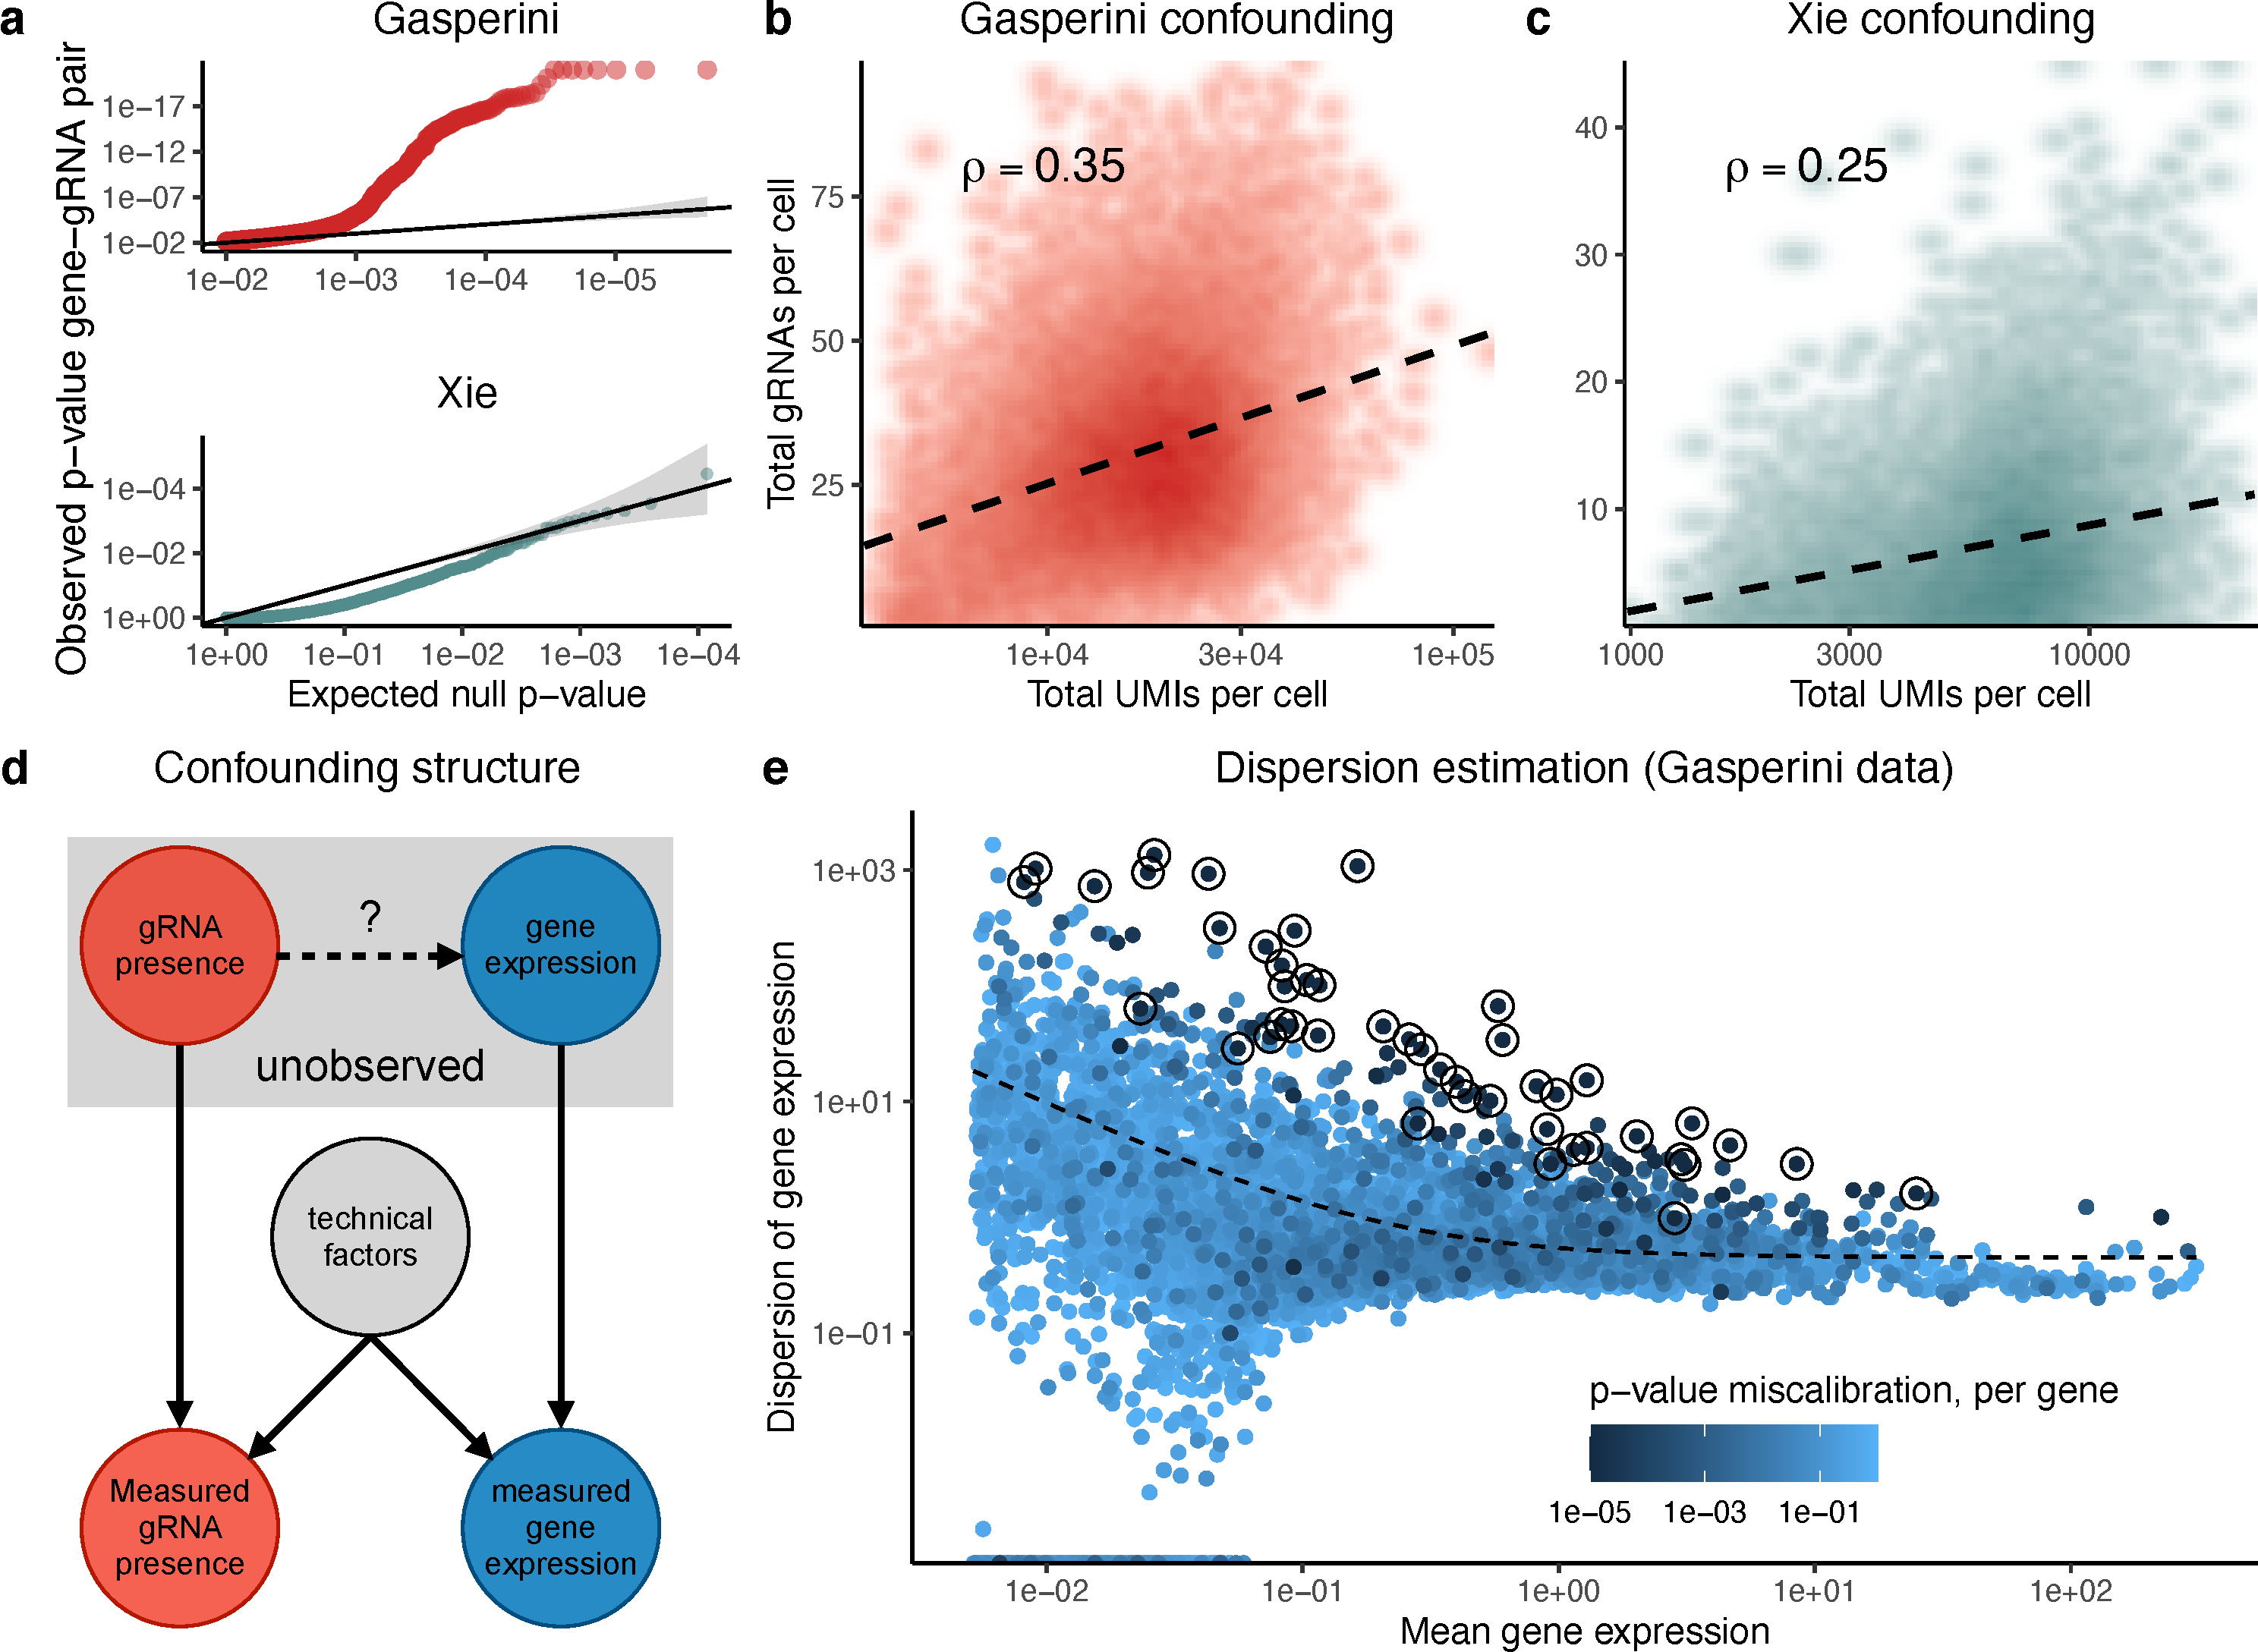
\includegraphics[width = \textwidth]{figures/Figure1/Figure1_cropped.pdf}
\caption{\textbf{CRISPR screen analysis challenges can lead to false positives and false negatives}. \textbf{a}, (Top) QQ-plot of Gasperini et al.\ p-values for all pairs of genes and negative control gRNAs. (Bottom) QQ-plot of Xie et al.\ p-values for all pairs of genes and ARL15-enh-targeting gRNAs (\textit{ARL15} gene omitted). These sets of $p$-values deviate from the expected uniform distribution, indicating test miscalibration. \textbf{b-d}, Sequencing depth (total mRNA UMIs per cell) impacts gRNA detection and observed gene expression levels in both Gasperini et al.\ (\textbf{b}) and Xie et al.\ (\textbf{c}) data. Thus, sequencing depth acts as a confounder (\textbf{d}). This analysis challenge distinguishes CRISPR screens from traditional differential expression applications. \textbf{e}, Monocle2 estimates the dispersion of each gene by projecting each gene's raw dispersion estimate onto the fitted raw dispersion-mean expression curve. This estimation procedure leads to miscalibration for high-dispersion genes.  % \textbf{b-c}, Sequencing depth (total mRNA UMIs per cell) impacts gRNA detection (b) and observed expression levels, and therefore acts as a confounder (c). This analysis challenge distinguishes CRISPR screens from traditional differential expression applications. }
}
 \label{fig:analysis-challenges}
\end{figure}
\clearpage

\paragraph{Improvements to the negative binomial approach.} 

We attempted to alleviate the miscalibration within the negative binomial regression framework. To this end, we followed the recommendations of Hafmeister and Satija, who recently proposed a strategy for parametric modeling of single cell RNA-seq data that, to the best of our knowledge, is state-of-the-art.\cite{Hafemeister2019}  First, we abandoned the DESeq2-style size factors of Monocle2 and instead corrected for sequencing depth by including sequencing depth as a covariate in the negative binomial regression model. Second, we adopted a more flexible dispersion estimation procedure. Following Hafmeister and Satija, we (i) computed raw dispersion estimates for each gene, (ii) regressed the raw dispersion estimates onto the mean gene expressions via kernel regression, and (iii) projected the raw dispersion estimates onto the fitted nonparametric regression curve.

We reanalyzed the Gasperini et al.\ data using the improved negative binomial regression approach. In addition to sequencing depth, we included as covariates in the regression model the total number of expressed genes per cell, as well as the technical factors that Gasperini et al.\ accounted for in their analysis (namely, total number of gRNAs detected per cell, percentage of transcripts mapped to mitochondrial genes, and sequencing batch). We also applied the improved negative binomial approach to the Xie et al.\ ARL15-enh data. In the latter analysis we included sequencing depth, number of detected gRNA UMIs per cell, and sequencing batch as covariates. We found that the improved negative binomial model was better calibrated than the Monocle2 negative binomial model on the Gasperini data (Figure 3c; improved negative binomial denoted ``Hafemeister NB''). However, on both the Gasperini et al.\ data and Xie et al.\ data, the improved negative binomial model showed clear signs of p-value inflation (Figure 3c-d).

There are many possible explanations for the remaining miscalibration, mostly due to misspecification of the negative binomial model. While more effort could be invested into further improvements of a parametric model for gene expression, modeling single cell data remains a challenging problem outside the scope of the current work. This difficulty highlights the appeal of nonparametric methods for singe cell analysis.\cite{Zhu2019} However, as discussed in the previous section, traditional nonparametric approaches are not applicable in the presence of technical factors that impact both gRNA detection and gene expression measurement. To resolve this impasse, we propose a resampling-based approach designed to account for such confounders.

% The difficulty of applying parametric models to single cell data highlights the appeal of nonparametric approaches for this purpose.
\clearpage
\paragraph{SCEPTRE: Analysis of single cell perturbation screens via conditional resampling.} 

Instead of treating cells symmetrically, we propose to estimate the probability a given gRNA will be observed in a given cell, based on that cell's technical factors. For example, this probability tends to be higher in cells with larger sequencing depths. We propose to generate a null distribution for a given gene and a given gRNA by independently resampling the gRNA assignments for each cell based on their respective perturbation probabilities (Figure~\ref{fig:method}). This scheme is an instance of the conditional randomization test (CRT), recently proposed by Cand\`{e}s et al.\cite{CetL16} In contrast to standard permutation tests, the CRT explicitly accounts for technical factors that vary from cell to cell.

To quantify the effect of a given gRNA on a given gene, we use the improved negative binomial regression statistic described above. This yields a $z$-value, which would typically be compared to a standard normal null distribution based on the parametric negative binomial model. Instead, we build a null distribution for this statistic via conditional resampling. To this end, we first fit a logistic regression model for the observation of the gRNA in a cell based on its technical factors, yielding a fitted probability for each cell. Then, we generate a large number of resampled datasets, where the expression and the technical factors stay the same, while the gRNA assignment is redrawn independently for each cell based on its fitted probability. The negative binomial $z$-value is then recomputed for each of these datasets, which comprise a null distribution (depicted as a gray histogram in Figure~\ref{fig:method}). The SCEPTRE $p$-value is defined as the left tail probability of the original $z$-value under this null distribution, for sensitivity to perturbations that decrease expression (the right tail could be used for screens targeting repressive elements). The conditional resampling null distribution can differ substantially from that based on the negative binomial model---for the same test statistic---depending on the extent of model misspecification (Figure~\ref{fig:NB-vs-CP}).

To mitigate the extra computational cost of resampling, we implemented several accelerations. We found that the skew-$t$ distribution, used by CRISPhieRmix\cite{Daley2018} for a different purpose, provided a good fit to the null histograms. We employed this skew-$t$ approximation to obtain precise $p$-values based on a limited number of resamples (500 in the current implementation). Furthermore, we implemented computational accelerations that reduced the cost of each resample by a factor of about 100 (see Methods). The original negative binomial regression takes about 3 seconds per gene-gRNA pair, while recomputing the test statistic for 500 resamples takes a total of 16 seconds. Therefore, SCEPTRE takes about 19 seconds per pair, compared to 3 seconds for the original method.

\clearpage
\thispagestyle{empty}
\begin{figure}[h!]
	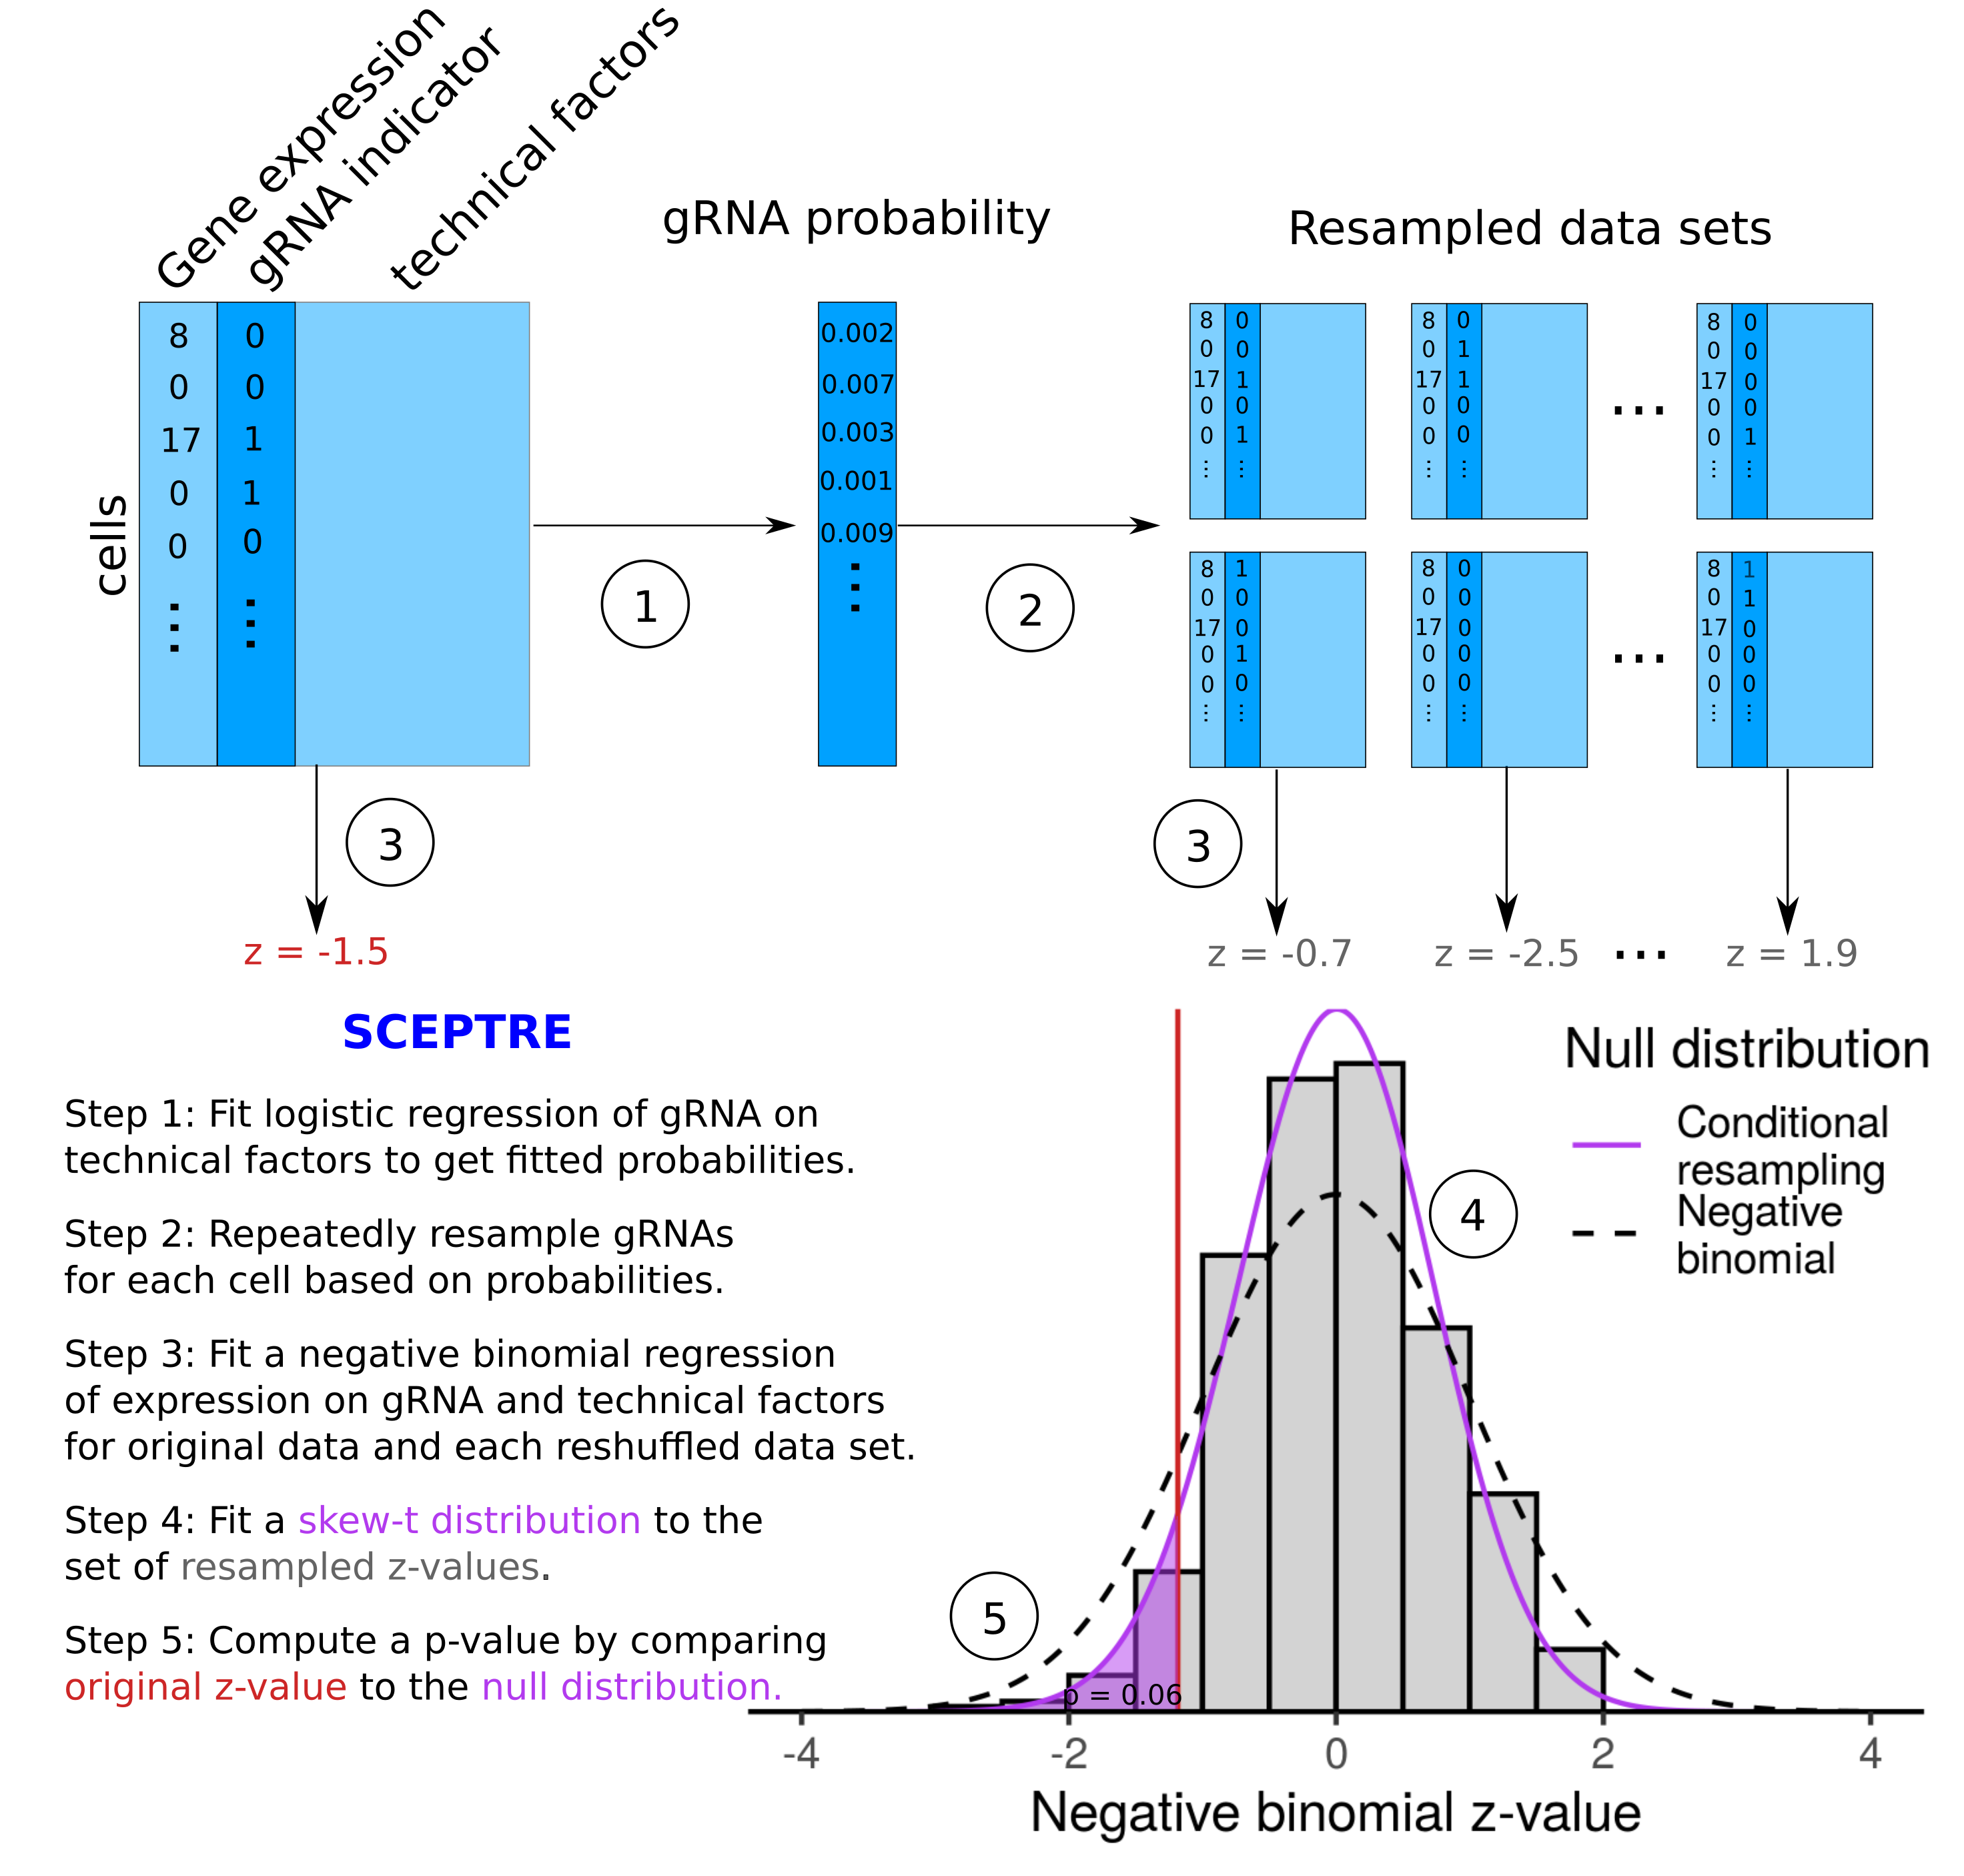
\includegraphics[width = \textwidth]{figures/Figure2/Figure2.png}
	\caption{\textbf{SCEPTRE: Analysis of single cell perturbation screens via conditional resampling.} A schematic and outline of the SCEPTRE methodology for one gene and one gRNA is shown, entailing the application of the conditional randomization test\cite{CetL16} to single cell CRISPR screens. The idea is to assign to every cell the probability of gRNA observation based on its technical factors, and then to build a null distribution for the negative binomial $z$-value by independently resampling the gRNA indicator for each cell according to these probabilities to form ``negative control" data sets. A skew-$t$ distribution is fit to the resulting histogram to obtain precise $p$-values based on a limited number of resamples, against which the original NB $z$-value is compared. The dashed line shows the standard normal distribution, against which the NB $z$-value would normally be compared.}
	\label{fig:method}
\end{figure}
\clearpage


\paragraph{SCEPTRE produces correct results when the ground truth is known.} 

We assessed the calibration, sensitivity, and specificity of SCEPTRE in several settings in which the ground truth was known. First, we demonstrated the calibration of SCEPTRE in a small, proof-of-concept simulation study (Figure \ref{fig:ground_truth}a). We considered a class of negative binomial regression models with dispersion $\alpha$ and two technical covariates (sequencing depth and batch). We simulated expression data for a single gene in 1000 cells using four models selected from this class: the first with $\alpha = 1$, the second with $\alpha = 0.25$, the third with $\alpha = 5$, and the last with $\alpha = 1,$ but with 25$\%$ zero-inflation. We also simulated negative control gRNA data using a logistic regression model with the same covariates as in the gene expression model. We assessed the calibration of three methods across the four simulated datasets: SCEPTRE, improved negative binomial regression, and scMAGeCK-LR,\cite{Yang2020} a recently-proposed, permutation-based nonparametric method. To assess the impact of model misspecification on SCEPTRE and the improved negative binomial method (on which SCEPTRE relies), we fixed the dispersion of the negative binomial method to 1 across all four simulated datasets. We found that the negative binomial method works as expected when the model is correctly specified but breaks down in all three cases of model misspecification. scMAGeCK-LR exhibits poor calibration across all simulated datasets, likely because, as a traditional nonparametric method, it fails to adequately account for confounders. Finally, SCEPTRE is well-calibrated regardless of expression model misspecification and confounder presence.

Next, to assess the calibration of SCEPTRE on real data, we applied SCEPTRE to test the association between all negative control gRNAs and all genes in the Gasperini et al.\ data (Figure \ref{fig:ground_truth}b) and all ARL15-enh-targeting gRNAs and all genes in the Xie et al.\ data (Figure \ref{fig:ground_truth}c). We compared SCEPTRE to the improved negative binomial method, as well as to the original analysis methods (i.e., Monocle regression on the Gasperini et al.\ data and Virtual FACS on the Xie et al.\ data). We did not apply scMAGeCK-LR to these data given its poor calibration on the simulated data. SCEPTRE shows excellent calibration on the Gasperini et al.\ negative control data; Monocle regression and improved negative binomial regression, in contrast, demonstrate signs of severe $p$-value inflation. Similarly, on the Xie et al.\ ARL15-enh data, SCEPTRE exhibits nearly perfect calibration, whereas Virtual FACS and the improved negative binomial method show conservative and liberal bias, respectively.

Last, we assessed the sensitivity of SCEPTRE using the Gasperini et al.\ positive control data and confirmatory bulk RNA-seq data produced by Xie et al. We applied SCEPTRE to the 381 positive control gRNA-gene pairs assayed in Gasperini et al.\ (Figure~\ref{fig:ground_truth}d), where each gRNA targeted the transcription start site of the corresponding gene. The SCEPTRE $p$-values for these positive controls are highly significant, and in particular, more significant than the original empirical $p$-values, indicating greater sensitivity. We note that the empirical correction employed by Gasperini et al.\ limits the accuracy of $p$-values to about $10^{-6}$, explaining at least part of the difference. Finally, we compared the SCEPTRE results for ARL15-enh to the results of an arrayed CRISPR screen of ARL15-enh in which populations of perturbed cells were compared to populations of unperturbed cells via bulk RNA-seq.\cite{Xie2019} Both SCEPTRE and the bulk RNA-seq differential expression analysis rejected gene \textit{ARL15} (and only gene \textit{ARL15}) at an FDR of 0.1 after a Benjamini-Hochberg correction, increasing our confidence in sensitivity (and specificity) of SCEPTRE (Figure \ref{fig:ground_truth}e).

\newpage
\begin{figure}[h!]
	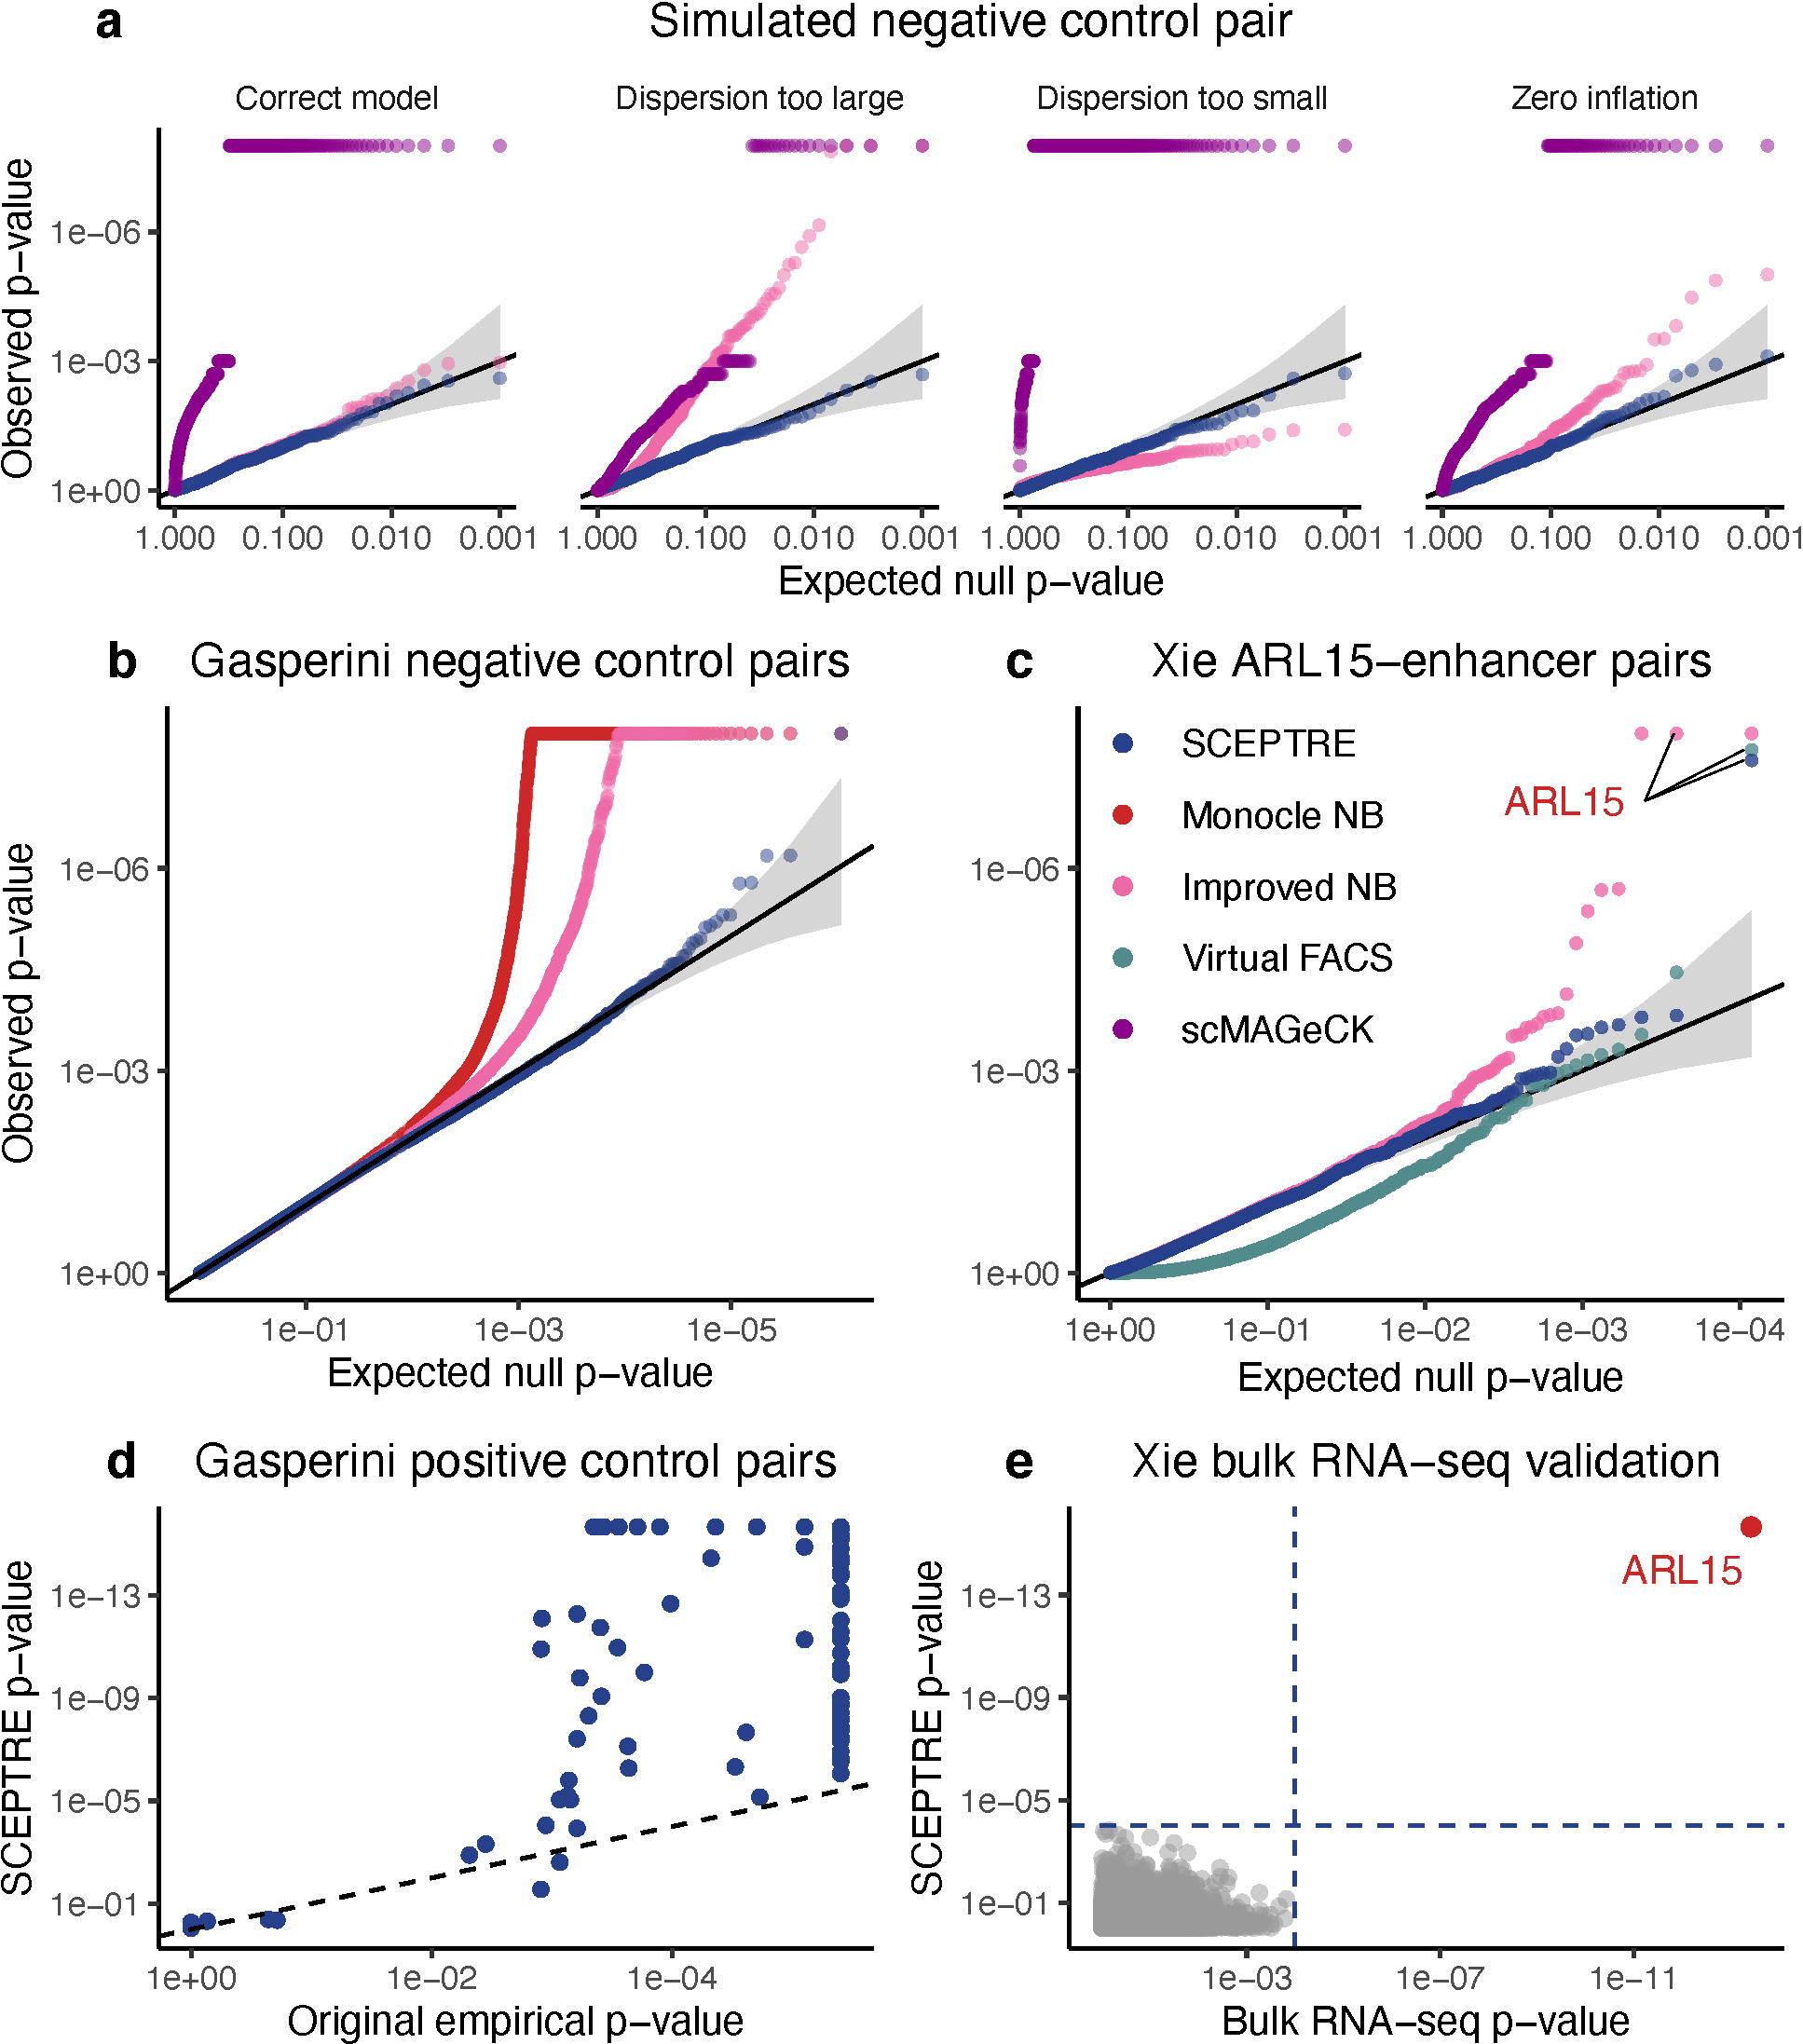
\includegraphics[width = \textwidth]{figures/Figure3/Figure3_cropped.pdf}
	\caption{\textbf{SCEPTRE demonstrates excellent calibration, specificity, and sensitivity when the ground truth is known.}}
	\label{fig:ground_truth}
 \end{figure}
\clearpage


% \clearpage
% \thispagestyle{empty} 
% \addtocounter{page}{-1}
%\begin{figure}[h!]
%	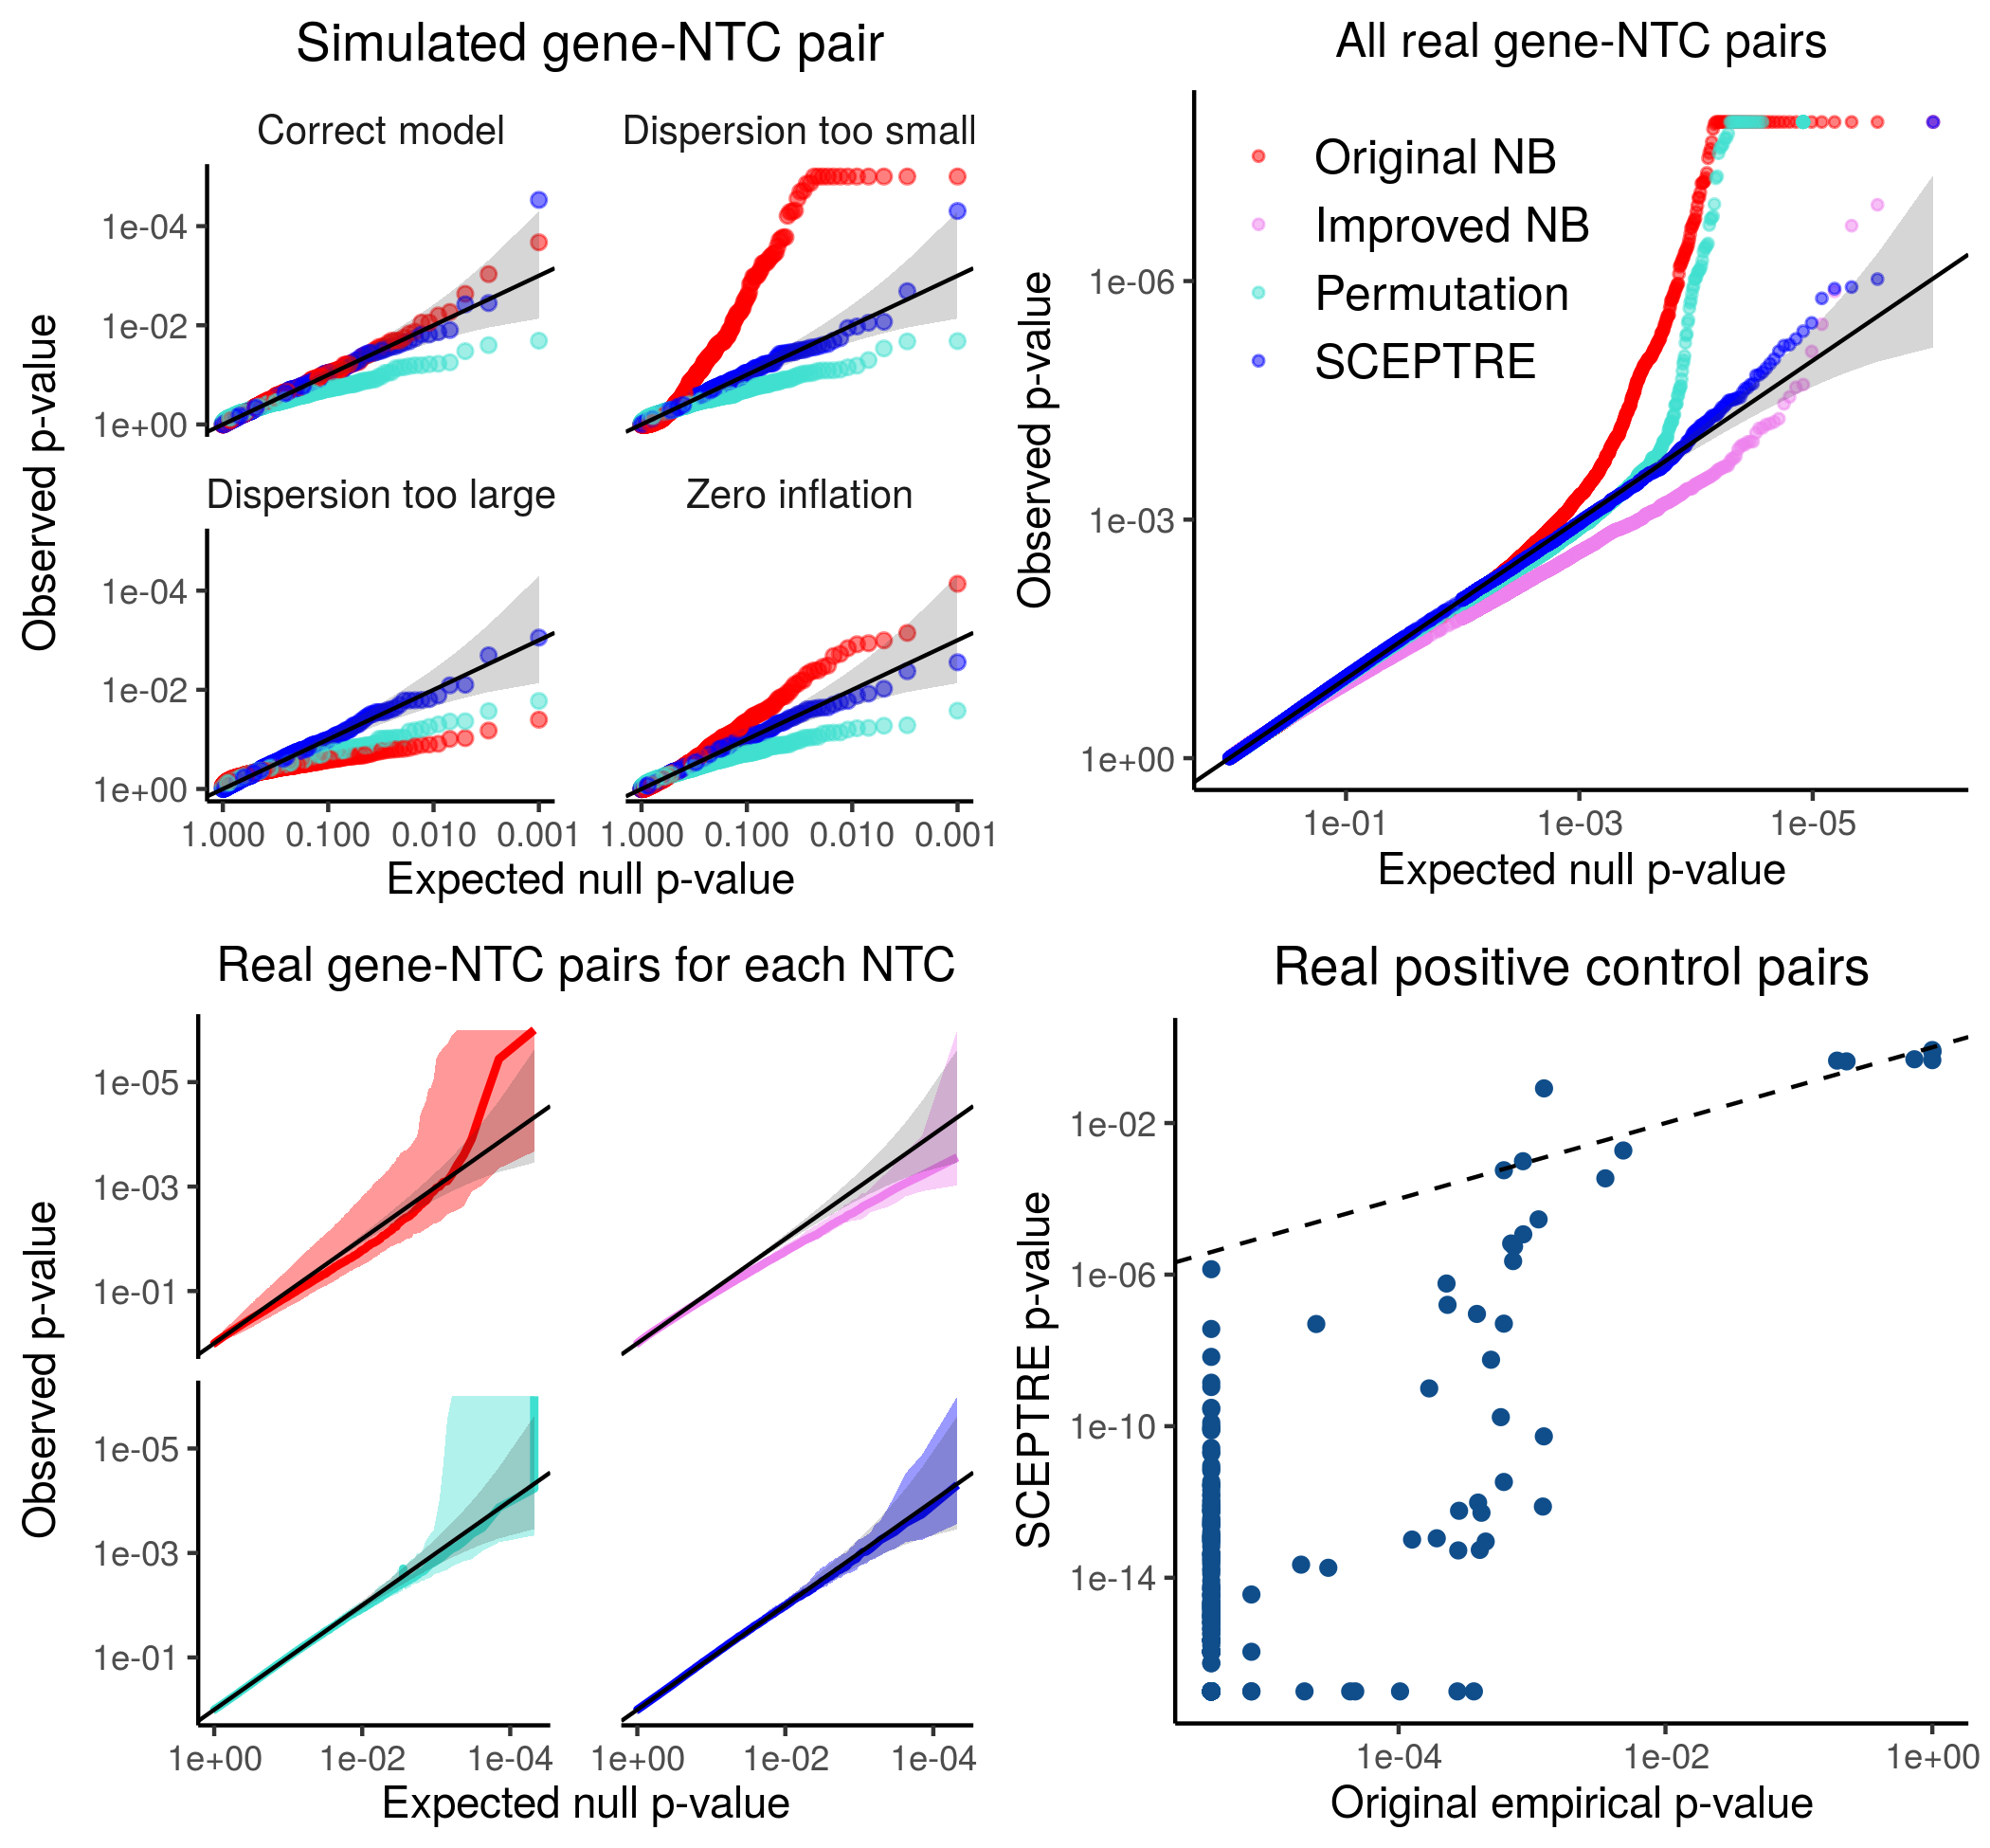
\includegraphics[width = \textwidth]{figures/Figure3/Figure3.png}
%	\caption{\textbf{SCEPTRE improves on the sensitivity and specificity of the parametric approach by correcting for expression model misspecification.} \textbf{a,} Numerical simulation comparing three ways of calibrating a negative binomial test statistic (parametric, permutation, conditional resampling), when the test statistic is based on the correct model or contains expression model misspecifications. Only the conditional resampling approach maintains calibration despite model misspecification. \textbf{b,c,} Application of SCEPTRE to Gasperini et al negative control gRNAs, comparing all gene-NTC pairs to the uniform distribution (b) or breaking down by NTC (c); details as in Figure~\ref{fig:calibration-comparison-all}a,c. The matching of SCEPTRE's colored region with the gray one in panel c, together with the overall near-uniformity in panel b, demonstrates its excellent calibration on real negative control data. \textbf{d,} SCEPTRE $p$-values for TSS-targeting controls generally more significant than the original empirical $p$-values; dashed line is the $45^\circ$ line. Note: $p$-values truncated for visualization, and empirical $p$-values in panel d at least 1/538,560 $\approx$ 2$\times 10^{-6}$ by construction.}
%	\label{fig:calibration}
% \end{figure}
\clearpage

\paragraph{Analysis of candidate gene-enhancer regulatory relationships.}

We applied SCEPTRE to the 84,595 gene-enhancer pairs considered in Gasperini et al., encompassing 10,560 genes and 5,779 candidate enhancers. We applied the Benjamini-Hochberg correction at level 0.1 (the same level used in the original analysis) to the $p$-values obtained for all of these candidate pairs, obtaining a total of 563 gene-enhancer pairs. By comparison, Gasperini et al. found 470 high-confidence pairs. Comparing the SCEPTRE $p$-values against the original empirical $p$-values (Figure~\ref{fig:application}a), we see that the two often diverge substantially. Our analysis found 200 gene-enhancer pairs that the original analysis did not, while 107 were found only by the original analysis. Many of the discoveries found only in the original analysis show signs of the $p$-value inflation observed in Figure~\ref{fig:analysis-challenges}. 

Among the 200 new gene-enhancer pairs discovered, several are supported by evidence from orthogonal functional assays. In particular, we highlight five of these pairs (Figure~\ref{fig:application}b) involving genes not paired to any enhancers in the original analysis, which are supported by GTEx\cite{GTExPilot} eQTL $p$-values in whole blood or enhancer RNA correlation $p$-values across tissues from the FANTOM project\cite{Andersson2014}. These pairs are listed in the GeneHancer database\cite{Fishilevich2017}, which aggregates eQTL, eRNA, and other sources of evidence of gene-enhancer interactions. The SCEPTRE $p$-values for these promising pairs are generally 1-2 orders of magnitude more significant than the original empirical $p$-values. Also among the 200 new gene-enhancer pairs are 6 pairs involving 5 genes that were deemed outliers in the original analysis (blue triangles in Figure~\ref{fig:application}a), underscoring SCEPTRE's ability to handle genes with arbitrary distributions that may not fit into traditional parametric models. 

We also found that the total set of gene-enhancer pairs discovered was better enriched for regulatory biological signals, including HI-C and ChIP-seq. Gene-enhancer pairs discovered by SCEPTRE tended to be physically closer to each other on average that those discovered in the original analysis (Figure~\ref{fig:application}c). Furthermore, 74.4\% of SCEPTRE's 563 gene-enhancer pairs fell in the same topologically associating domain (TAD), compared to 71.1\% of the original 470 pairs. We also repeated Gasperini et al.'s contact frequency enrichment analysis for those pairs falling in the same TAD (Figure~\ref{fig:application}d). We found similar levels of contact frequency enrichment, despite the fact that SCEPTRE discovered 85 more gene-enhancer pairs in the same TADs. Finally, we repeated the ChIP-seq enrichment analysis of Gasperini et al. for seven cell-type relevant transcription factors and H3K27ac. We quantified enrichment of ChIP-seq signal in paired enhancers as the odds ratio that a candidate enhancer is paired to a gene, comparing those falling in the top quintile of candidate enhancers by ChIP-seq signal and those not overlapping a ChIP-seq peak at all. We find improved enrichment for each of the eight ChIP-seq targets (Figures~\ref{fig:application}e and \ref{fig:chipseq-enrichment-details}).

\clearpage
% \newgeometry{top=0.6in}
% \thispagestyle{empty} 
% \addtocounter{page}{-1}
% \vspace{-2in}
% \begin{figure}
%	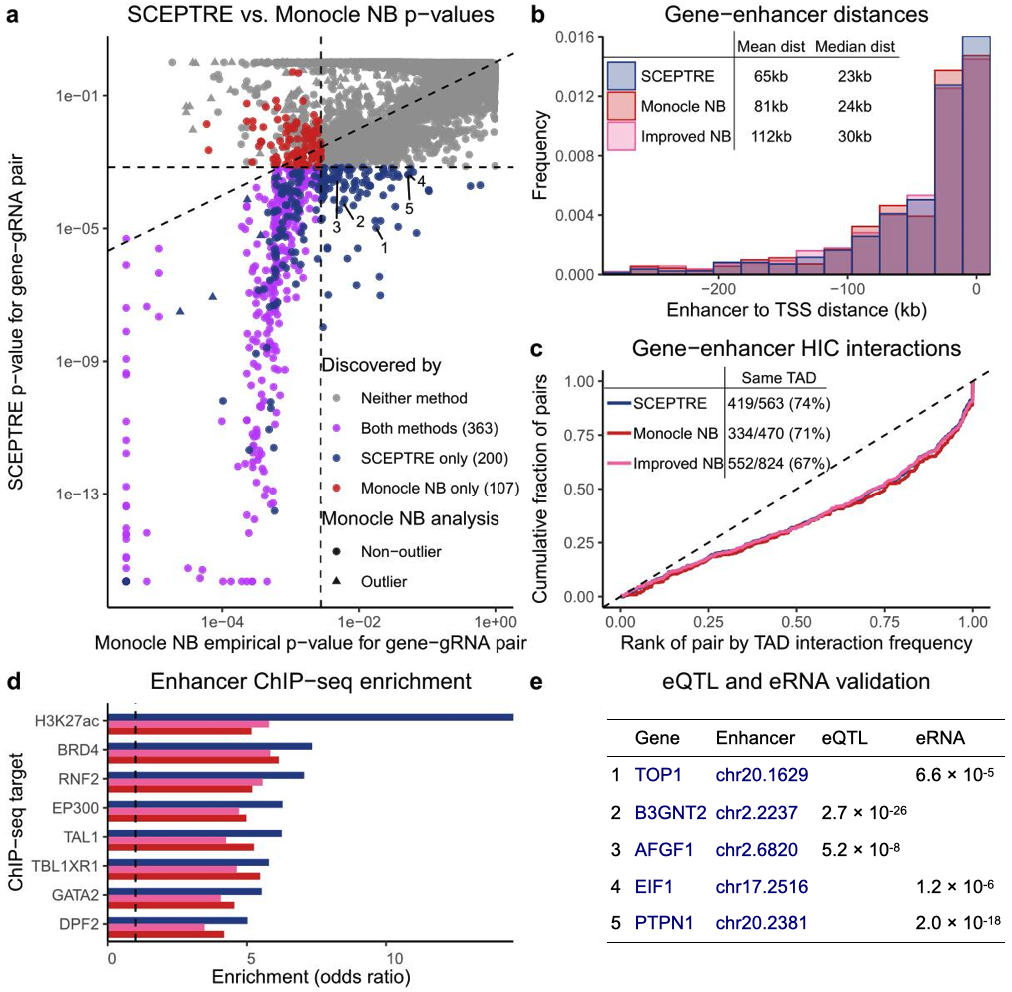
\includegraphics[width = \textwidth]{figures/Figure4/Figure4.png}
%	\caption{\textbf{Application to Gasperini et al. data yields biologically plausible gene-enhancer links.}  \textbf{a,} Well-calibrated NTC $p$-values give confidence in SCEPTRE $p$-values for candidate enhancers (compare to Figure~\ref{fig:analysis-challenges}a). \textbf{b}, Comparing the original empirical $p$-values to those obtained from SCEPTRE. The two analysis methods differ substantially, with 217 gene-enhancer links discovered only by SCEPTRE and 102 discovered only by the original. \textbf{c}, Five gene-enhancer pairs discovered by SCEPTRE but not the original analysis, each supported by a whole blood GTEx eQTL or FANTOM enhancer RNA correlation $p$-value. \textbf{d,} Distribution of distances from TSS to upstream paired enhancers. Compared to the original analysis, SCEPTRE pairs genes with nearer enhancers on average. \textbf{e,} For those gene-enhancer pairs falling in the same TAD, the cumulative distribution of the fractional rank of the HI-C interaction frequency compared to other distance-matched loci pairs within the same TAD. SCEPTRE shows similar enrichment despite finding 32\% more within-TAD pairs. Inset table shows gene-enhancer pairs falling in the same TAD. SCEPTRE finds 115 more total pairs, and a higher percentage of pairs fall in the same TAD. \textbf{f,} Enrichment of ChIP-seq signal from seven cell-type relevant transcription factors and one histone mark among paired enhancers. SCEPTRE exhibits greater enrichment across all ChIP-seq targets.}
%	\label{fig:application}
% \end{figure}

\begin{figure}
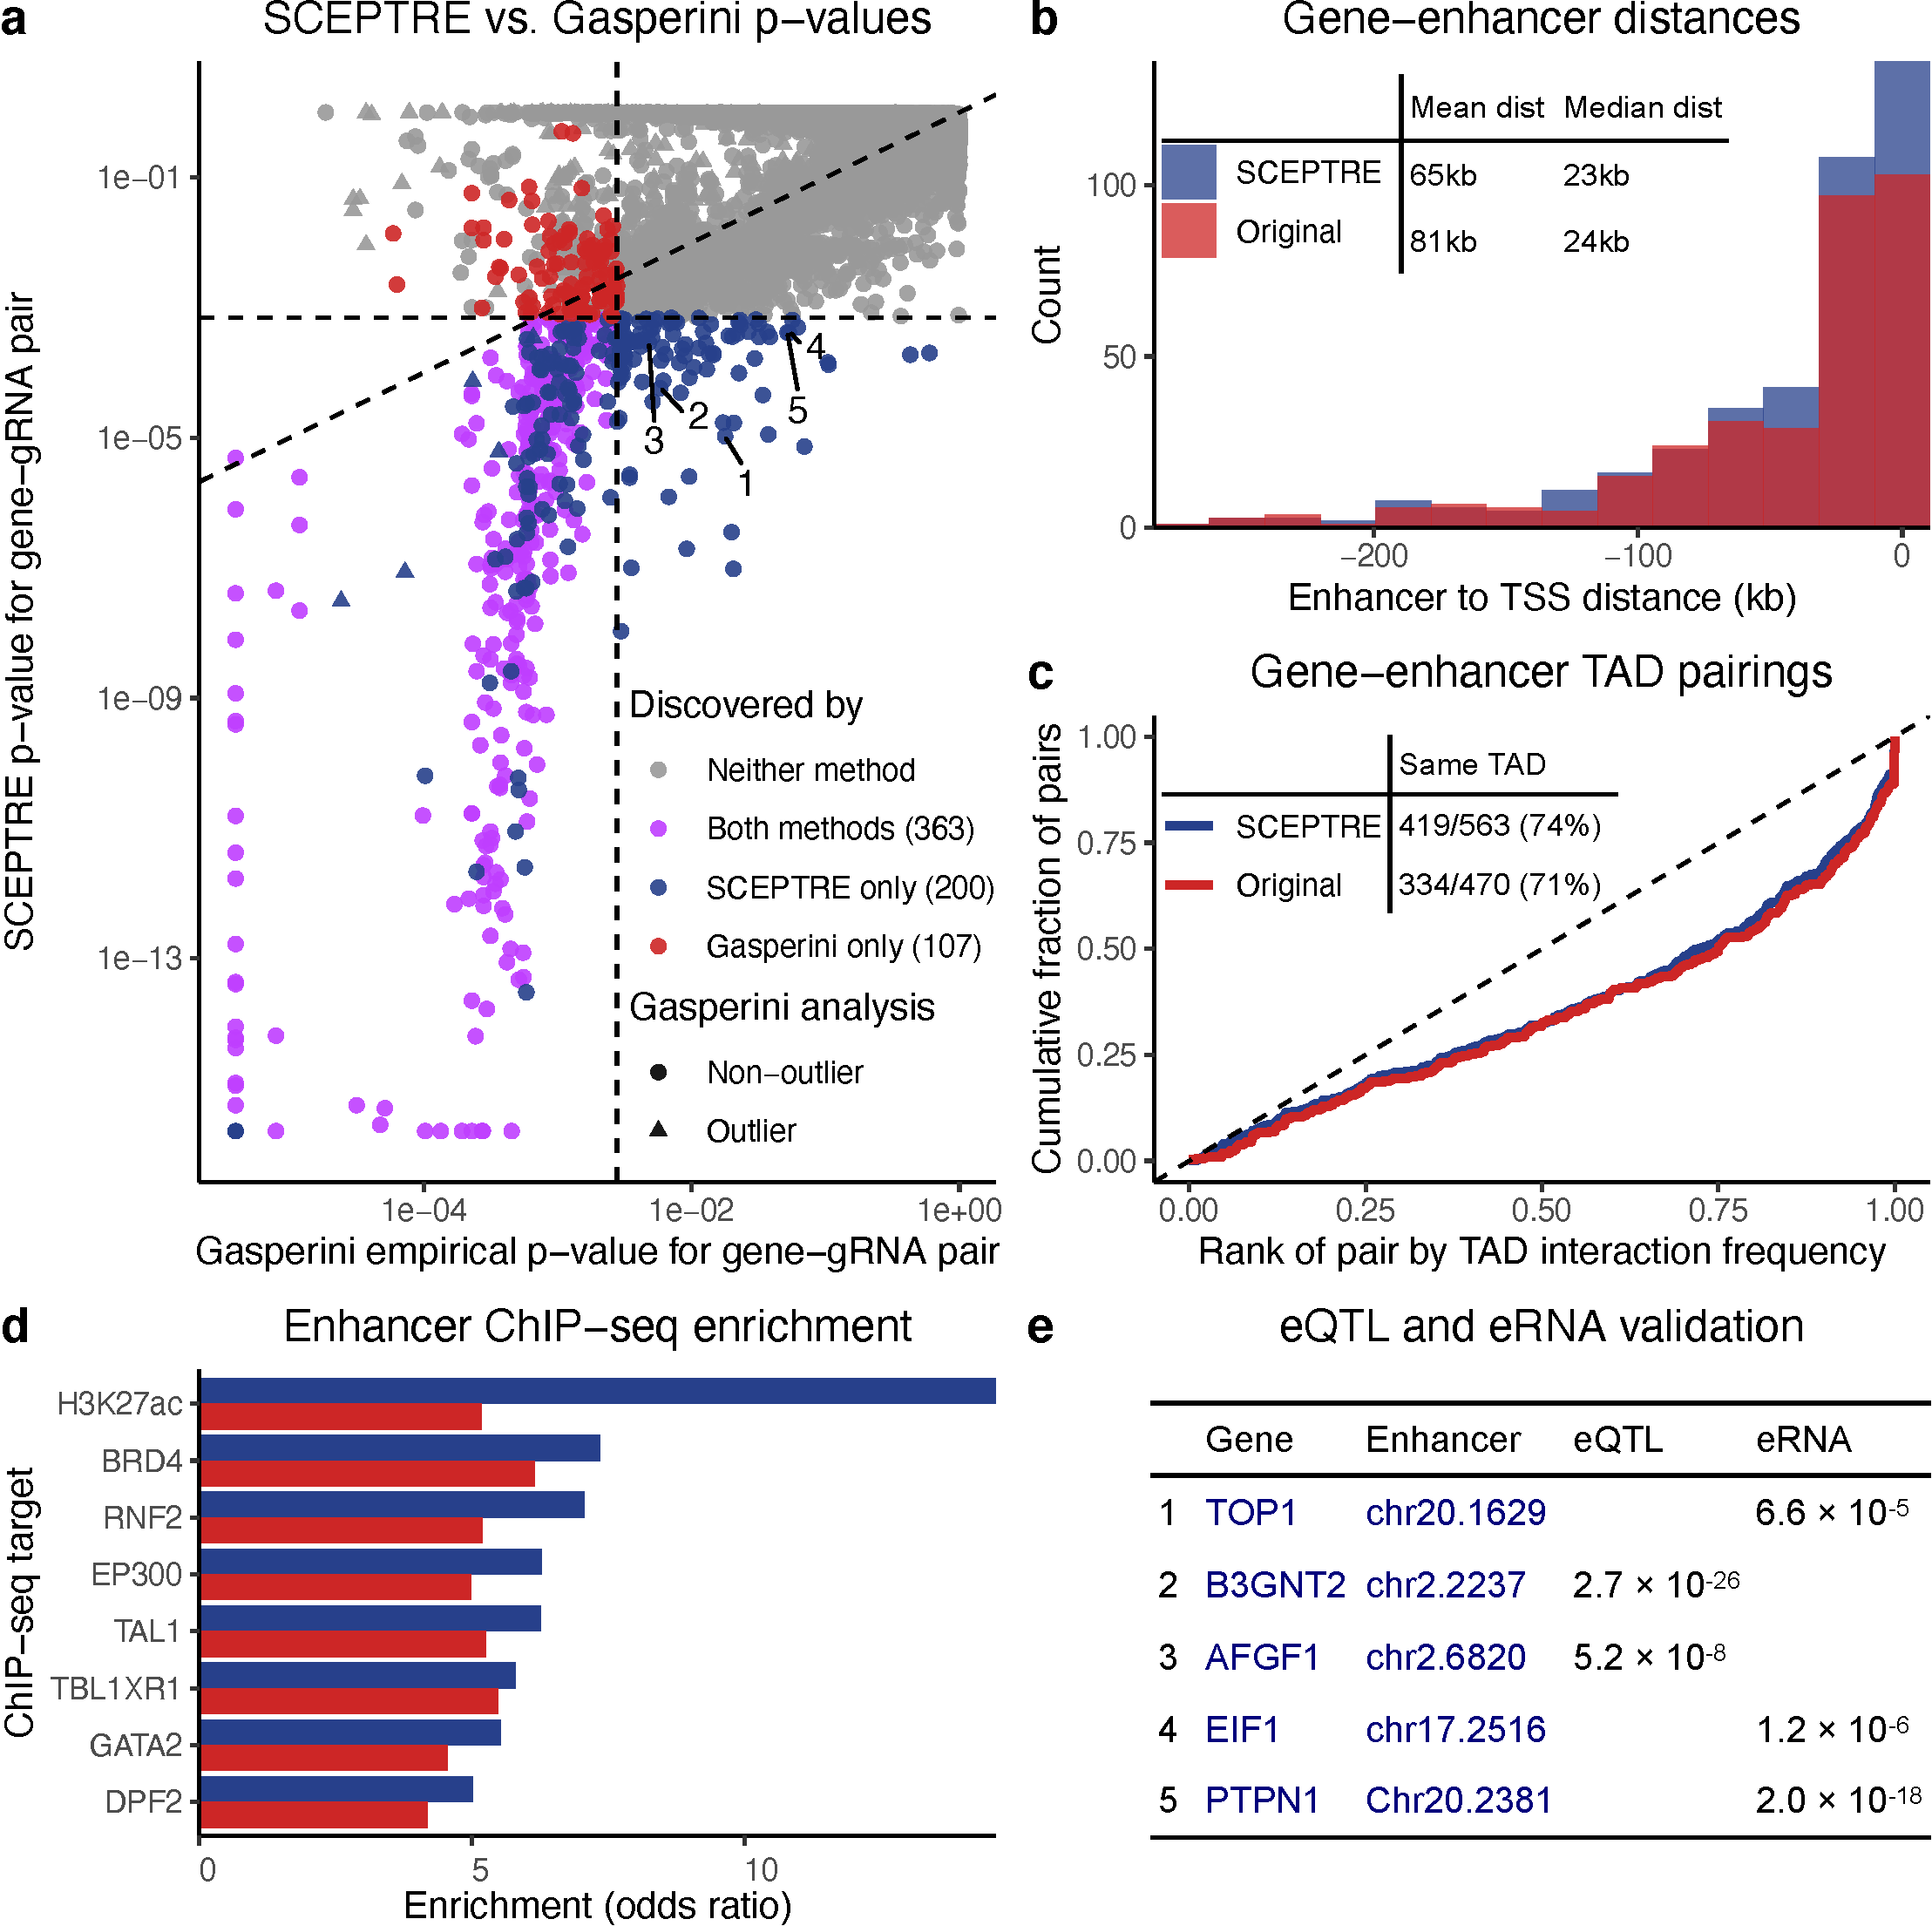
\includegraphics[width = \textwidth]{figures/Figure4/Figure4_cropped.pdf}
	\caption{\textbf{Application to Gasperini et al. data yields biologically plausible gene-enhancer links.} }
	\label{fig:application}
\end{figure}

\clearpage
% \restoregeometry


\section*{Discussion}

Here we illustrate a variety of statistical challenges arising in the analysis of single cell CRISPR screens, leaving existing methods (based on parametric expression models, permutations, or negative control data) vulnerable to calibration issues. To address these challenges, we develop SCEPTRE, a novel resampling method based on modeling the probability a given gRNA will be observed in a given cell, based on that cell's technical factors. SCEPTRE exhibits excellent calibration despite the presence of confounding technical factors and despite misspecification of single cell gene expression models. We implement computational accelerations to bring the cost of our resampling-based methodology down to well within an order of magnitude of the traditional approach, making it quite feasible to apply for large-scale data. We use SCEPTRE to reanalyze the Gasperini et al. data and a subset of the Xie et al. data, yielding many new biologically plausible gene-enhancer relationships supported by evidence from eQTL, enhancer RNA co-expression, ChIP-seq, and HI-C data. 

The main assumption behind SCEPTRE's validity is the accuracy of the model for gRNA observation. Our calibration results suggest that this is a reasonable assumption for the simulated and negative control data considered here. However, more work is necessary to assess the quality of gRNA measurement models across a broader range of contexts. Furthermore, we conjecture that misspecifications in the gRNA measurement model can be compensated by improved gene expression models, a statistical phenomenon referred to as ``double robustness"\cite{Robins2001,VanderLaan2003}. Better expression models can also improve the sensitivity of the conditional randomization test\cite{Katsevich2020a}.

There are several directions for improvement in the analysis of single cell CRISPR screens, which are not addressed by SCEPTRE. Many of these have been considered before, especially in the context of non-single-cell CRISPR screens. Such remaining challenges include variable effectiveness of gRNAs\cite{Li2015,Daley2018,Xie2019}, interactions among perturbed elements\cite{Xie2017,Zamanighomi2019,Norman2019}, and the limited resolution of CRISPR interference\cite{Hsu2018}. Additionally, single cell CRISPR screens would benefit from the adoption of techniques from the increasingly rich literature on scRNA-seq analysis. 

The conditional resampling methodology underlying SCEPTRE is extremely flexible, paving the way for its applicability to future iterations of CRISPR screens and beyond. For example, direct capture Perturb-seq\cite{Replogle2020} has recently been proposed in order to improve the efficiency of gRNA detection. However, the capture rate can vary substantially across gRNAs. We look forward to adapting the SCEPTRE framework to the analysis of such new CRISPR screen technologies. Finally, confounding technical factors like those pictured in Figure~\ref{fig:analysis-challenges}c are ubiquitous across genomics; we anticipate the conditional randomization test will complement traditional parametric and nonparametric methods in such contexts as a valuable analysis tool.

\bibliography{library}

\clearpage

\begin{addendum}
 \item We are indebted to Molly Gasperini, Jacob Tome, and Andrew Hill for clarifying several aspects of their data analysis\cite{Gasperini2019} and to the Shendure lab for providing extensive feedback on an earlier draft of this paper. We thank Shiqi Xie for providing guidance on using the Xie et al.\ 2019 data, Wie Li for a helpful discussion on scMAGeCK, and John Morris for providing feedback on the SCEPTRE code. Finally, we thank Tom Norman, Atray Dixit, and Wesley Tansey for useful discussions on single cell CRISPR screens. This work was supported, in part, by National Institute of Mental Health (NIMH) grants R01MH123184 and R37MH057881 as well as SFARI Grant 575547. Part of the data analysis used the Extreme Science and Engineering Discovery Environment (XSEDE)\cite{XSEDE}, which is supported by National Science Foundation grant number ACI-1548562. Specifically, it used the Bridges system\cite{Bridges}, which is supported by NSF award number ACI-1445606, at the Pittsburgh Supercomputing Center (PSC). \item[Competing Interests] The authors declare that they have no
competing financial interests.
 \item[Correspondence] Correspondence and requests for materials
should be addressed to E.K. \\ (email: ekatsevi@wharton.upenn.edu).
\end{addendum}


\section*{Methods}

\paragraph{Conditional randomization test.}
Consider a particular gene/gRNA pair. For each cell $i = 1, \dots, n$, let $X_i \in \{0,1\}$ indicate whether the gRNA was present in the cell, let $Y_i \in \{0,1,2,\dots\}$ be the gene expression in the cell, defined as the number of unique molecular identifiers (UMIs) from this gene, and let $Z_i \in \mathbb R^d$ be a list of cell-level technical factors. Letting $(X, Y, Z) = \{(X_i, Y_i, Z_i)\}_{i = 1}^{n}$, consider any test statistic $T(X,Y,Z)$ measuring the effect of the gRNA on the expression of the gene. The conditional randomization test\cite{CetL16} is based on resampling the gRNA indicators independently for each cell. Letting $\pi_i = \mathbb P[X_i = 1 | Z_i]$, define random variables
\begin{equation}
\widetilde X_i \overset{\text{ind}}\sim \text{Ber}(\pi_i). 
\label{X-tilde-dist}
\end{equation}
Then, the CRT $p$-value is given by
\begin{equation}
p_{\text{CRT}} = \mathbb P[T(\widetilde X, Y, Z) \geq T(X,Y,Z)\mid X,Y,Z].
\label{conditional-randomization}
\end{equation}
This translates to repeatedly sampling $\widetilde X$ from the distribution~\eqref{X-tilde-dist}, recomputing the test statistic with $X$ replaced by $\widetilde X$, and defining the $p$-value as the probability the resampled test statistic exceeds the original. Under the null hypothesis that the gRNA perturbation does not impact the cell (adjusting for technical factors), i.e. $Y \independent X \mid Z$, we obtain a valid $p$-value~\eqref{conditional-randomization}, \textit{regardless of the expression distribution $Y|X,Z$ and regardless of the test statistic $T$}. We choose as a test statistic $T$ the $z$-score of $X_i$ obtained from a negative binomial regression of $Y_i$ on $X_i$ and $Z_i$:

\begin{equation}
Y_i \overset{\text{ind}} \sim \text{NegBin}(\mu_i, \alpha); \quad \log(\mu_i) = \beta_0 + X_i \beta + Z_i^T \gamma
\label{negative-binomial},
\end{equation}
where $\alpha$ is the dispersion. Following Hafemeister and Satjia\cite{Hafemeister2019}, we estimate $\alpha$ by pooling dispersion information across genes, and we include sequencing depth as an entry in the vector of technical factors  $Z_i$ (see section \textit{Improvements to the negative binomial approach}).

\paragraph{Accelerations to the conditional randomization test.}
We implemented computational accelerations to the conditional randomization test. First, we employed the recently proposed\cite{Liu2020} \textit{distillation} technique to accelerate the recomputation of the negative binomial regression for each resample. The idea is to use a slightly modified test statistic, consisting of two steps:
\begin{enumerate}
	\item Fit $(\widehat \beta_0, \widehat \gamma)$ from the negative binomial regression~\eqref{negative-binomial} except without the gRNA term:
	\begin{equation}
	Y_i \overset{\text{ind}}\sim \textrm{NegBin}(\mu_i, \alpha); \quad \log(\mu_i) = \beta_0 + Z_i^T \gamma.
	\label{negative-binomial-distillation}
	\end{equation}
	\item Fit $\widehat \beta$ from a negative binomial regression with the estimated contributions of $Z_i$ from step 1 as offsets:
	\begin{equation}
	Y_i \overset{\text{ind}}\sim \textrm{NegBin}(\mu_i, \alpha); \quad \log(\mu_i) = X_i \beta + \widehat \beta_0 + Z_i^T \widehat \gamma.
	\label{distilled-negative-binomial}
	\end{equation}
\end{enumerate}
Conditional randomization testing with this two step test statistic, which is nearly identical to the full negative binomial regression~\eqref{negative-binomial}, is much faster. Indeed, since the first step is not a function of $X_i$, it remains the same for each resampled triple $(\widetilde X, Y, Z)$. Therefore, only the second step must be recomputed with each resample, and this step is faster because it involves only a univariate regression.

Next, we accelerated the second step above using the sparsity of the binary vector $(X_1, \dots, X_n)$ (or a resample of it). To do so, we wrote the log-likelihood of the reduced negative binomial regression~\eqref{distilled-negative-binomial} as follows, denoting by $\ell(Y_i, \log(\mu_i))$ the negative binomial log-likelihood:
\begin{equation*}
\begin{split}
\sum_{i = 1}^n \ell(Y_i, X_i \beta + \widehat \beta_0 + Z_i^T \widehat \gamma) &= \sum_{i: X_i = 0} \ell(Y_i, \widehat \beta_0 + Z_i^T \widehat \gamma) + \sum_{i: X_i = 1} \ell(Y_i, \beta + \widehat \beta_0 + Z_i^T \widehat \gamma) \\
&= C + \sum_{i: X_i = 1} \ell(Y_i, \beta + \widehat \beta_0 + Z_i^T \widehat \gamma).
\end{split}
\end{equation*}
This simple calculation shows that, up to a constant that does not depend on $\beta$, the negative binomial log-likelihood corresponding to the model~\eqref{distilled-negative-binomial} is the same as that corresponding to the model with only intercept and offset term for those cells with a gRNA:
\begin{equation}
Y_i \overset{\text{ind}}\sim \textrm{NegBin}(\mu_i, \alpha); \quad \log(\mu_i) = \beta + \widehat \beta_0 + Z_i^T \widehat \gamma, \quad \text{for } i \text{ such that } X_i = 1.
\label{distilled-negative-binomial-accelerated}
\end{equation}
The above negative binomial regression is therefore equivalent to equation~\eqref{distilled-negative-binomial}, but much faster to compute, because it involves only the thousand or so cells containing the gRNA instead of the 200,000 total cells.

\paragraph{SCEPTRE methodology.}

In practice, we must estimate the gRNA probabilities $\pi_i$ as well as the $p$-value $p_{\text{CRT}}$. This is because usually we do not know the distribution $X|Z$, and cannot compute the conditional probability in equation~\eqref{conditional-randomization} exactly. We propose to estimate $\pi_i$ via logistic regression of $X$ on $Z$, and to estimate $p_{\text{CRT}}$ by resampling $\widetilde X$ a large number of times and then fitting a skew-$t$ distribution to the resampling null distribution $T(\widetilde X, Y, Z)|X,Y,Z$. We outline SCEPTRE below: 
\begin{enumerate}
	\item Fit technical factor effects $(\widehat \beta_0,\widehat \gamma)$ on gene expression using the negative binomial regression~\eqref{negative-binomial-distillation}.
	\item Extract a $z$-score $z(X,Y,Z)$ from the reduced negative binomial regression~\eqref{distilled-negative-binomial-accelerated}.
	\item Assume that 
	\begin{equation}
	X_i \overset{\text{ind}}\sim \text{Ber}(\pi_i); \quad \log\left(\frac{\pi_i}{1-\pi_i}\right) = \tau_0 + Z_i^T \tau
	\label{logistic-regression}
	\end{equation}
	for $\tau_0 \in \mathbb R$ and $\tau \in \mathbb R^d$, and fit $(\widehat \tau_0, \widehat \tau)$ via logistic regression of $X$ on $Z$. Then, extract the fitted probabilities $\widehat \pi_i = (1+\exp(-(\widehat \tau_0 + Z_i^T \widehat \tau)))^{-1}$.	
	\item For $b = 1, \dots, B$,
	\begin{itemize}
		\item Resample the gRNA assignments based on the probabilities $\widehat \pi_i$ to obtain $\widetilde X^b$~\eqref{X-tilde-dist}.
		\item Extract a $z$-score $z(\widetilde X^b, Y, Z)$ from the reduced negative binomial regression~\eqref{distilled-negative-binomial-accelerated}.
	\end{itemize}
	\item Fit a skew-$t$ distribution $\widehat F_{\text{null}}$ to the resampled $z$-scores $\{z(\widetilde X^b, Y, Z)\}_{b = 1}^B$. 
	\item Return the $p$-value $\widehat p_{\text{SCEPTRE}} = \mathbb P[\widehat F_{\text{null}} \leq z(X,Y,Z)]$.
\end{enumerate}
In our data analysis, we used $B = 500$ resamples. Following Gasperini et al.\, we based our analysis on the top two gRNAs targeting each enhancer. Some enhancers were also targeted with two additional gRNAs, but we excluded these from the analysis.

\paragraph{Numerical simulation to assess calibration.}

We simulated one gene $Y_i,$ five gRNAs $X_{i1}, X_{i2}, \dots, X_{i5},$ and two confounders $Z_{i1}, Z_{i2}$ in $n = 1000$ cells. We generated the confounders $Z_{i1}$ and $Z_{i2}$ by sampling with replacement the sequence batch IDs and log-transformed sequencing depths, respectively, of the cells in the Gasperini dataset. The batch ID confounder $Z_{i1}$ was a binary variable, as the Gasperni data included two batches. Next, we drew the gRNA indicators $X_{i1}, X_{i2}, \dots, X_{i5}$ i.i.d.\ from the logistic regression model (7), with $\tau_0 = -7, \tau_1 = -2,$ and $\tau_2 = 0.5$. We selected these parameters to make the probability of gRNA occurrence about 0.04 across cells. Finally, we drew the gene expression $Y_i$ from the following zero-inflated negative binomial model:
$$ Y_i \sim \lambda \delta_0 + (1 - \lambda) \textrm{NegBin}(\mu_i, \alpha), \textrm{ } \log(\mu_i) = \beta_0 + Z_i^T \beta.$$ Note that gRNA presence or absence does not impact gene expression in this model. 
We set $\beta_0 = -2.5, \beta_1 = -2, \beta_2 = 0.5$ to make the average gene expression about $4$ across cells. We generated the four datasets shown in Figure \ref{fig:ground_truth}a by setting the dispersion parameter $\alpha$ and the zero inflation rate parameter $\lambda$ equal to the following values:
$$ (\lambda_1, \alpha_1) = (0,1) ; \textrm{    } (\lambda_2, \alpha_2) = (0, 5); \textrm{     } (\lambda_3, \alpha_3) = (0, 0.2); \textrm{     } (\lambda_4, \alpha_4) = (0.25, 1).$$ For the first, the negative binomial model is correctly specified. For the second and third, the dispersion estimate of 1 is too small and too large, respectively. The last setting exhibits zero inflation

We applied SCEPTRE, negative binomial regression, and scMAGeCK-LR\cite{Yang2020} to the four problem settings, each with $n_{sim} = 500$ repetitions. The negative binomial method was based on the $z$ statistic from the Hafemeister-inspired negative binomial model (\ref{negative-binomial}) with $\alpha = 1$.  scMAGeCK-LR differs from SCEPTRE and the negative binomial method in that scMAGeCK-LR computes $p$-values for all enhancers simultaneously. Thus, to facilitate comparisons across methods, we plotted $p$-values corresponding to enhancer $X_{i1}$ only. We used $B = 500$ resamples for SCEPTRE and $B = 1000$ permutations for scMAGeCK-LR, the default choices for these methods.

\paragraph{Definition of Gasperini et al. discovery set.}

Gasperini et al. reported a total of 664 gene-enhancer pairs, identifying 470 of these as ``high-confidence." We chose to use the latter set, rather than the former, for all our comparisons. Gasperini et al. carried out their ChIP-seq and HI-C enrichment analyses only on the high-confidence discoveries, so for those comparisons we do the same. Furthermore, the 664 total gene-enhancer pairs reported in the original analysis were the result of a Benjamini-Hochberg FDR correction that included not only the candidate enhancers but also hundreds of positive controls. While Bonferroni corrections can only become more conservative when including more hypotheses, BH corrections are known to become anticonservative when extra positive controls are included\cite{FR01}. To avoid this extra risk of false positives, we chose to use the ``high-confidence" set throughout.

\paragraph{ChIP-seq, HI-C enrichment analyses.}

ChIP-seq and HI-C enrichment analyses analyses (see Figures~\ref{fig:application}e-f and \ref{fig:chipseq-enrichment-details}) were carried out almost exactly following Gasperini et al. The only change we made is in our quantification of the ChIP-seq enrichment (Figure~\ref{fig:application}f). We use the odds ratio of a candidate enhancer being paired to a gene, comparing the top and bottom ChIP-seq quintiles.

\section*{Data availability}

Analysis results are available online at \url{https://bit.ly/SCEPTRE}. All analysis was performed on publicly available data. The CRISPR screen data\cite{Gasperini2019} is available at \url{https://www.ncbi.nlm.nih.gov/geo/query/acc.cgi?acc=GSE120861}. The ChIP-seq data are drawn from the ENCODE project\cite{Dunham2012} and are available at \url{https://www.encodeproject.org/}. The HI-C enrichment analysis is based on the data from Rao et al\cite{Rao2014}, available at \url{https://www.ncbi.nlm.nih.gov/geo/query/acc.cgi?acc=GSE63525}. The eQTL and eRNA co-expression $p$-values are taken from the GeneHancer database\cite{Fishilevich2017}, available as part of GeneCards (\url{https://www.genecards.org/}).

\section*{Code availability}

Code to reproduce all data analysis is available on Github at \url{https://github.com/ekatsevi/SCEPTRE}.

\clearpage 

\appendix
%\newgeometry{top=1in}
% \thispagestyle{empty} 
% \addtocounter{page}{-1}

% \counterwithin{figure}{section}
\section{Supplementary Figures}
\renewcommand{\thesection}{S}

\vspace{0.25in}

%\clearpage

%\makeatletter 
%\renewcommand{\thefigure}{S\@arabic\c@figure}
%\makeatother


%\section*{Supplementary Figures}
\thispagestyle{empty}
%\vspace{-0.1in}
%\setcounter{figure}{0}    
%\renewcommand{\thefigure}{S\arabic{figure}}

%\begin{figure}[h!]
%	\centering
%	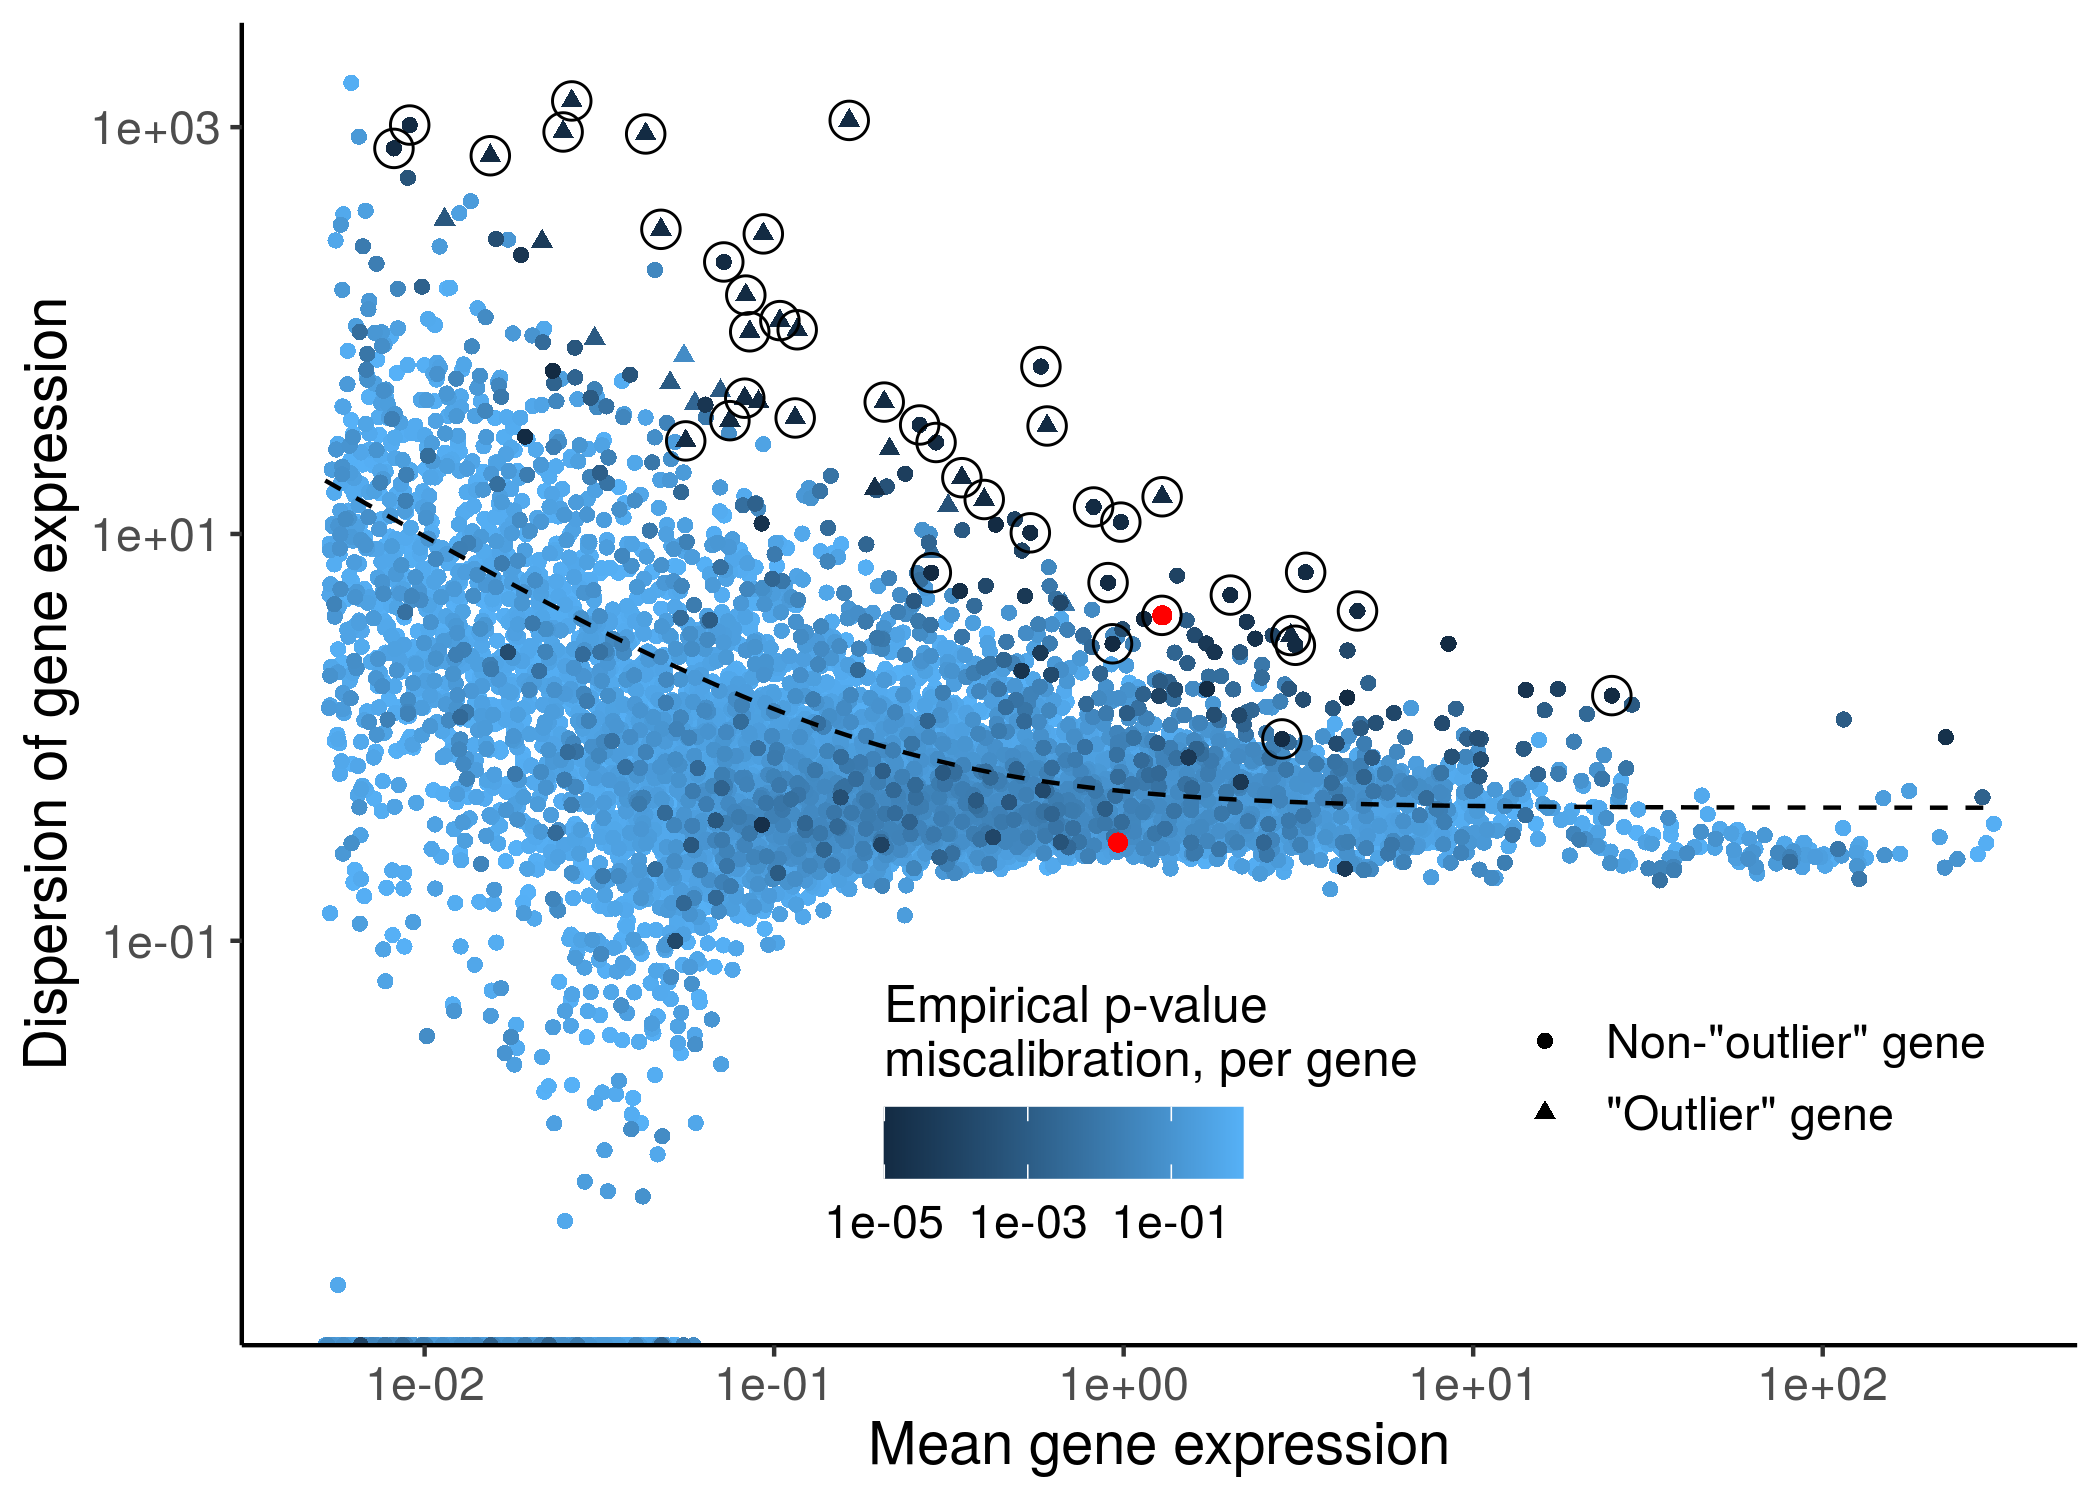
\includegraphics[width = \textwidth]{figures/FigureS1/FigureS1.png}
%	\caption{Gasperini et al.'s empirical correction is insufficient to correct for miscalibration. \textbf{a,} Dispersion estimation procedure employed leads to miscalibration for high-dispersion genes, which the empirical correction does not adequately correct for, as measured by KS test applied to empirical $p$-values per gene (point colors). \textbf{b,} Raw $p$-values already well-calibrated for LUC7L2 gene, so empirical correction unnecessarily shrinks the significance of the association with TSS-targeting gRNA, depicted by horizontal lines, by three orders of magnitude. \textbf{c,} Empirical correction not strong enough for HIST1H1D, which is among circled genes in panel a, which have an NTC-based miscalibration $p$-value smaller than the Bonferroni threshold. \textbf{d}, Under-correction leads to two potential false discoveries for HIST1H1D. Dashed horizontal line represents the multiple testing threshold.}
%	\label{fig:mosaicseq}
% \end{figure}

\clearpage

% \thispagestyle{empty} 
% \begin{figure}[h!]
%	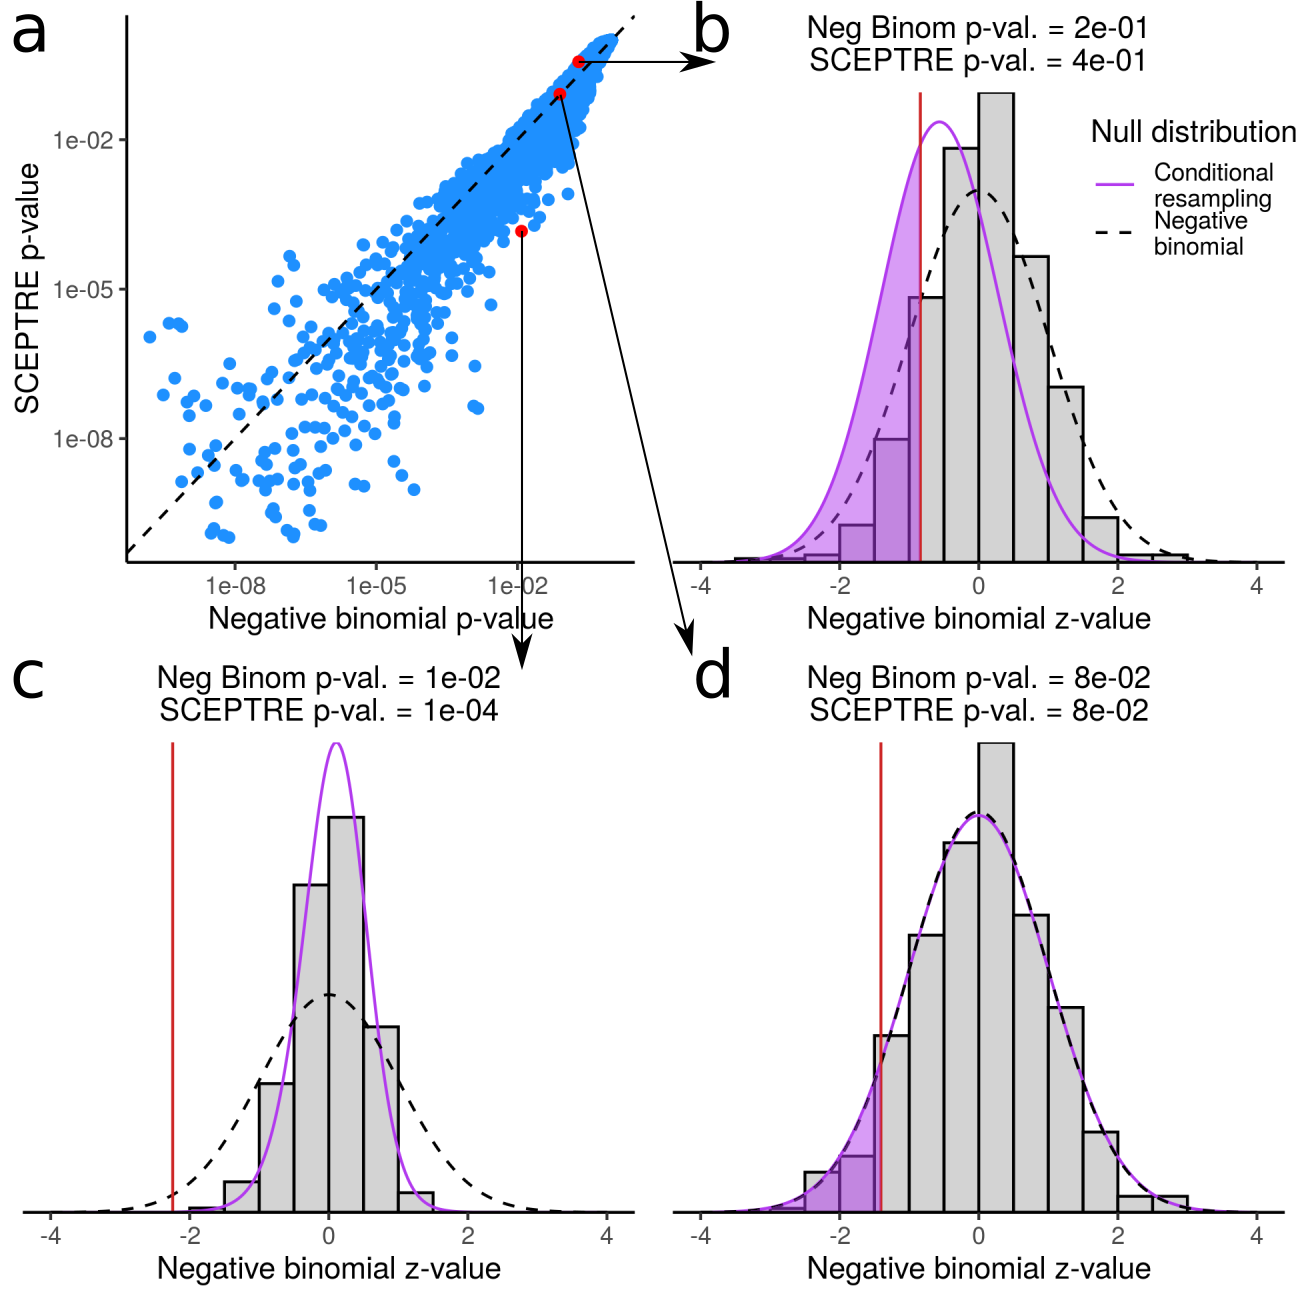
\includegraphics[width = \textwidth]{figures/FigureS2/FigureS2.png}
%	\caption{\textbf{Comparing negative binomial and conditional resampling $p$-values based on the same test statistic.} \textbf{a,} The standard parametric negative binomial $p$-value versus that obtained from the same test statistic by conditional resampling, for each gene / candidate enhancer pair (both truncated at $10^{-10}$ for visualization). The two can diverge fairly substantially. \textbf{b-d,} Parametric and conditional resampling null distributions for the negative binomial $z$-value in three cases: the parametric $p$-value is more significant (b), the conditional resampling $p$-value is more significant (c), the two $p$-values are about the same (d).}
%	\label{fig:NB-vs-CP}
% \end{figure}

%\restoregeometry



% \clearpage
% \thispagestyle{empty} 
% \begin{figure}[h!]
%	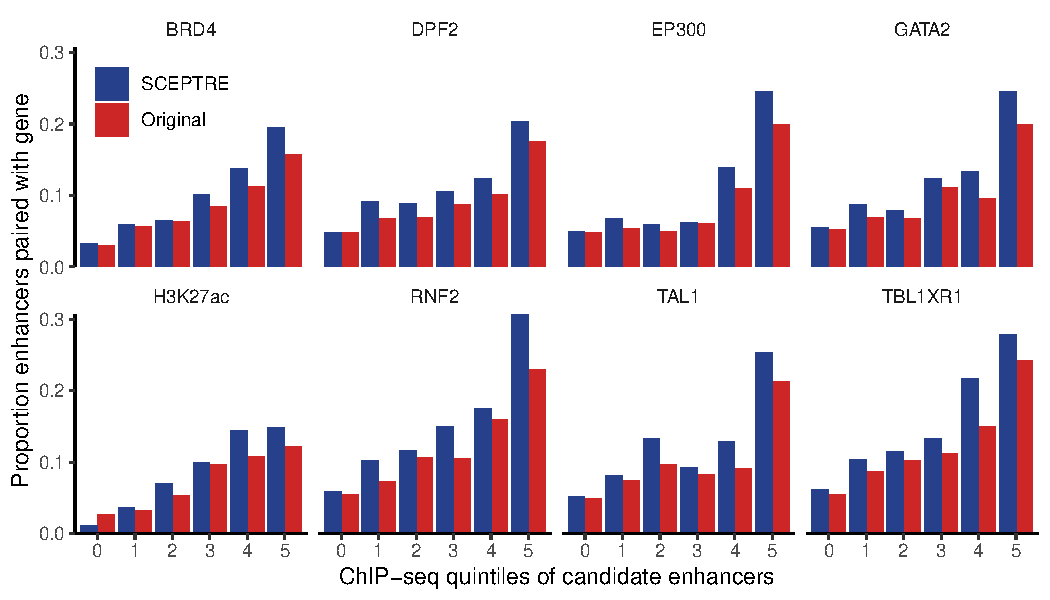
\includegraphics[width = \textwidth]{figures/FigureS3/FigureS3.pdf}
%	\caption{\textbf{Details on ChIP-seq enrichment analysis.} Fraction of candidate enhancers paired with a gene, broken down by quintile of ChIP-seq signal (0 means the candidate enhancer did not overlap a ChIP-seq peak), based on which the odds ratios in Figure~\ref{fig:application}f were computed. Both methods generally pair candidate enhancers in higher ChIP-seq quintiles more frequently, but this enrichment is more pronounced in SCEPTRE across all eight ChIP-seq targets.}
%	\label{fig:chipseq-enrichment-details}
% \end{figure}



\end{document}
